\chapter{耳蜗的听觉处理} \label{chap:chap26}
人类的经验因能够区分各种不同的声音而变得丰富——从耳语的亲切感到谈话的热情,从交响乐的复杂性到体育场的轰鸣声。 
当耳蜗的感觉细胞(内耳的感受器官)将声能转换为电信号并将其转发给大脑时,听力就开始了。 
我们识别声音细微差异的能力源于耳蜗区分频率分量、振幅和相对时间的能力。

听力取决于毛细胞的显着特性,毛细胞是内耳的细胞麦克风。 
毛细胞将声音引起的机械振动转换为电信号,然后将其传递给大脑进行解释。 
毛细胞可以测量原子尺寸的运动,并转换从静态输入到频率为数十千赫兹的刺激。 
值得注意的是,毛细胞还可以充当增强听觉灵敏度的机械放大器。 
每对耳蜗都含有大约 16,000 个这样的细胞。 
毛细胞及其神经支配的退化是造成工业化国家约 10\% 人口听力损失的主要原因。



\section{耳朵具有三个功能部分}
声音由弹性介质(空气)以大约 340 m/s 速度传播的交替压缩和稀疏性组成。 
这种压力变化波携带的机械能源于我们的发声器官或其他声源对空气产生的功。 
机械能被捕获并传输到受体器官,在那里它被转换成适合神经分析的电信号。 
这三个任务分别与外耳、中耳和内耳的耳蜗相关(图 26-1)。


\begin{figure}[htbp]
	\centering
	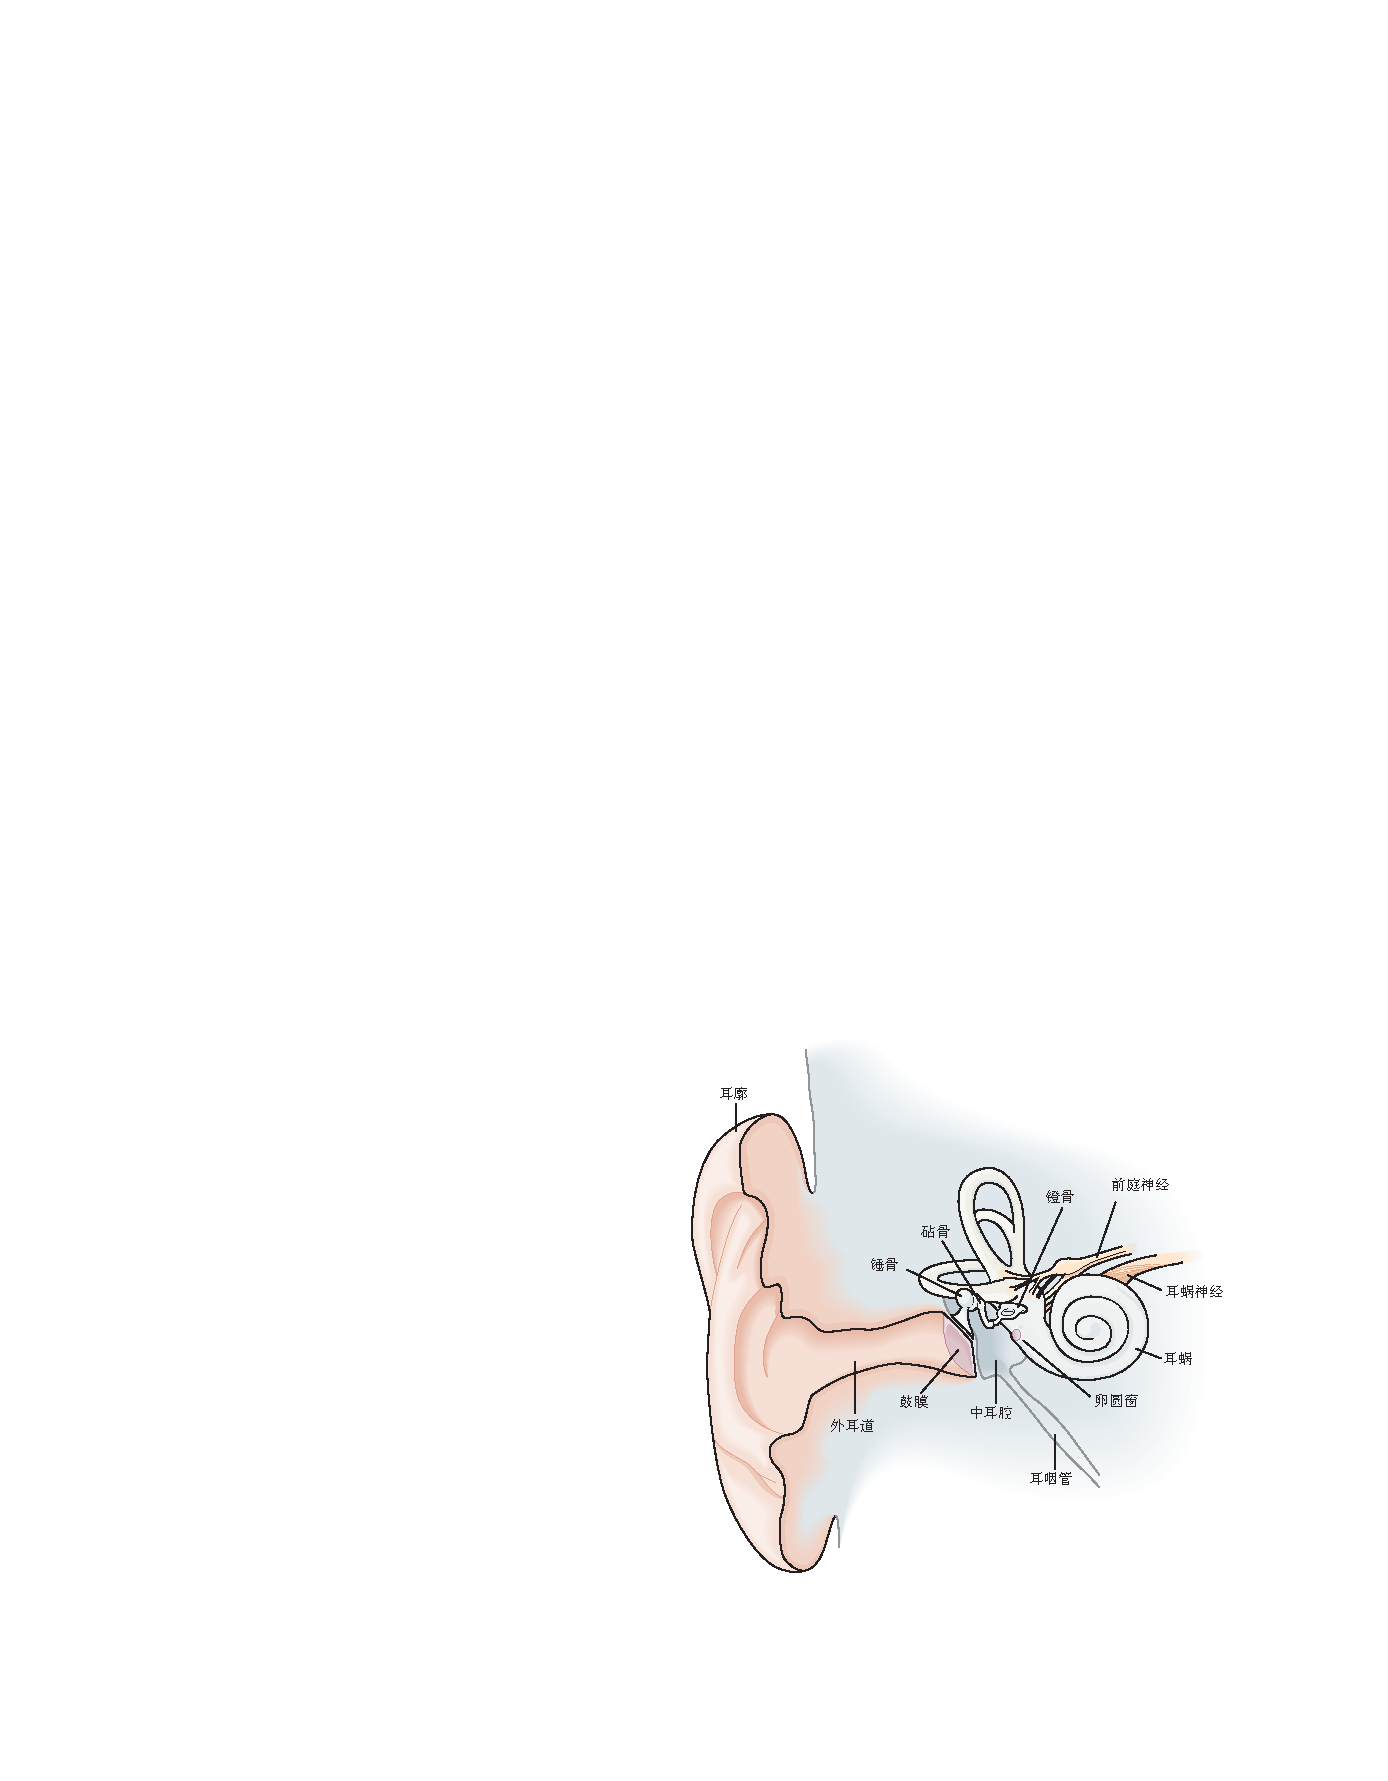
\includegraphics[width=0.5\linewidth]{chap26/fig_26_1}
	\caption{人耳的结构。 
		外耳,尤其是突出的耳廓,将声音聚焦到外耳道。 气压的交替升高和降低会振动鼓膜。 这些振动通过三块相连的小骨头传递到充满空气的中耳:锤骨、砧骨和镫骨。 
		镫骨的振动刺激内耳的听觉器官耳蜗。}
	\label{fig:26_1}
\end{figure}

人类外耳最明显的组成部分是耳廓,它是软骨支撑的皮肤的突出褶皱。 
耳廓充当反射器,可有效捕获声音并将其聚焦到外耳道或耳道中。 
耳道终止于鼓膜或鼓膜,这是一个直径约 9 毫米、厚度约 50 微米的隔膜。

外耳在捕捉来自各个方向的声音时的效果并不一致; 当声音起源于相对于头部的不同但特定的位置时,耳廓的波纹表面可以最好地收集声音。 
我们在空间中定位声音的能力,尤其是在垂直轴上,关键取决于这些声音收集特性。 
每个耳廓都有独特的地形; 它对不同频率声音反射的影响是大脑在生命早期就学会的。

中耳是一个充气袋,通过耳咽管与咽部相连。 
% 寒衣处处催刀尺,白帝城高急暮砧。——杜甫《秋兴八首(其一)》: 捣衣石
空气传播的声音作为听小骨的振动穿过中耳,听小骨是连接在一起的三块小骨头:锤骨(形似锤子)、砧骨(形似砧板)和镫骨(形似马镫,如图\ref{fig:26_1}所示)。 
锤骨的长延伸附着在鼓膜上; 它的另一端与砧骨有韧带连接,砧骨同样与镫骨相连。 
镫骨的扁平基部,即足板,位于耳蜗骨质覆盖物的开口(椭圆形窗口)中。 
听小骨是进化的遗迹。 
镫骨最初是古代鱼类鳃支撑的组成部分; 
锤骨和砧骨是爬行动物祖先的主要下颌关节的组成部分。


内耳包括听觉感觉器官,即耳蜗(形似蜗牛),一种直径逐渐减小的盘绕结构,缠绕在锥形骨核周围(图~\ref{fig:26_1})。 
在人类中,耳蜗大约有 9 毫米宽,有鹰嘴豆那么大,并嵌在颞骨内。 
耳蜗内部由三个平行的充满液体的隔室组成,称为阶梯。
在沿其螺旋路线的任何位置的耳蜗横截面中,顶部隔室是前庭阶(图~\ref{fig:26_2})。
在这个腔室的宽底端是椭圆形窗口,开口由镫骨的脚板密封。 
底部隔间是鼓阶; 它也有一个底部孔径,即圆窗,由一个薄而有弹性的膜片关闭,中耳腔的空气就在膜片之外。 
这两个腔室沿其大部分长度被耳蜗隔板隔开,但在耳蜗的最尖端通过螺旋体相互连通。

\begin{figure}[htbp]
	\centering
	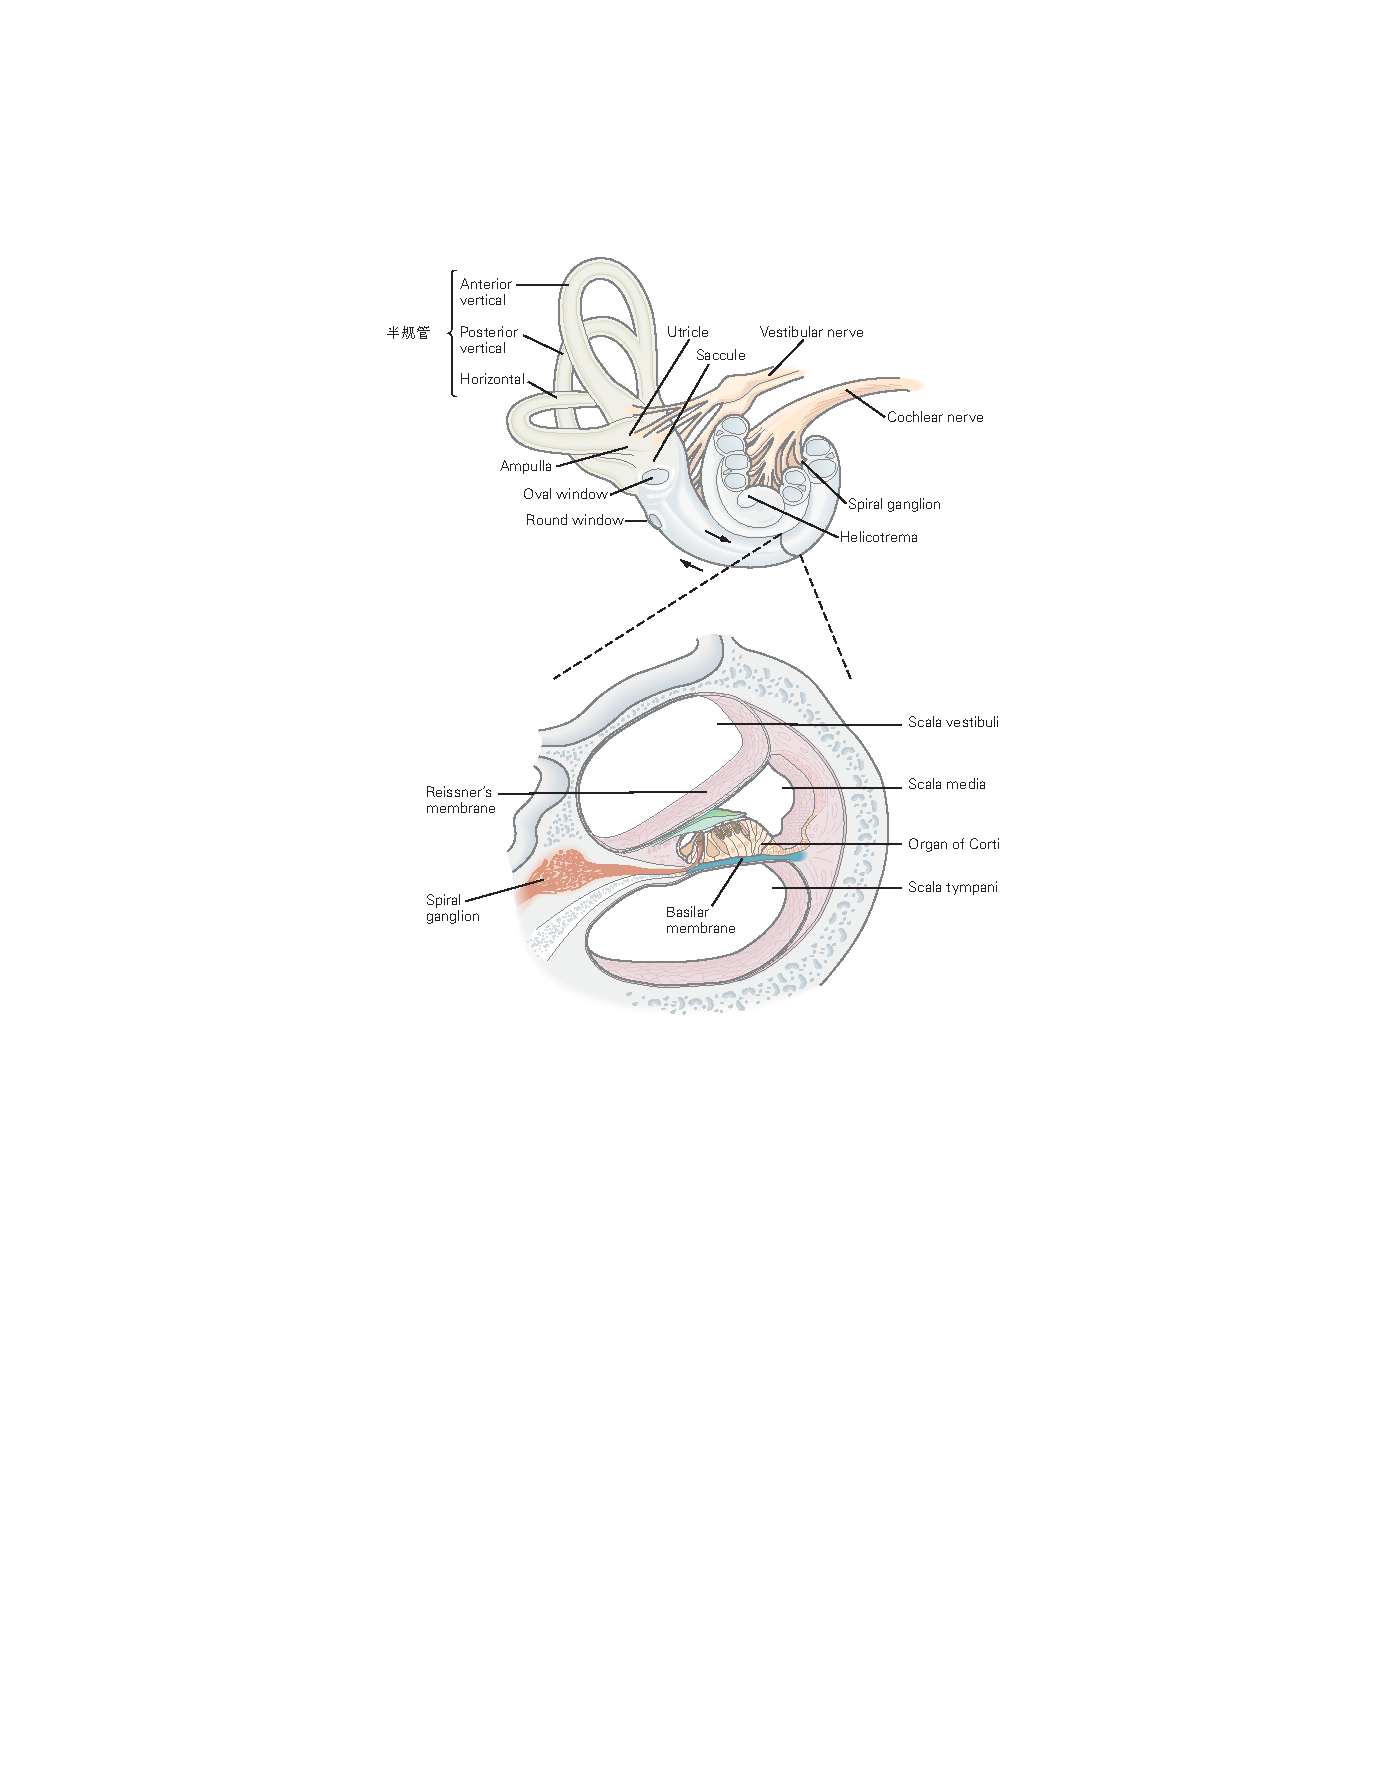
\includegraphics[width=0.5\linewidth]{chap26/fig_26_2}
	\caption{耳蜗的结构。 
		耳蜗的横截面显示了三个充满液体的导管或鳞片的排列,每个导管或鳞片长约 33 毫米。 
		前庭阶和鼓阶通过耳蜗顶端的螺旋体相通。 
		在底部,每个管道都由一个密封孔封闭。 
		前庭阶被椭圆窗关闭,镫骨响应声音推动它; 鼓阶由圆窗关闭,圆窗是一种薄而柔韧的膜。 
		在这两个隔间之间是阶中层,这是一个充满内淋巴的管,其上皮衬里包括位于基底膜(蓝色)上方的柯蒂氏器官中的 16,000 个毛细胞。 
		毛细胞被盖膜(绿色)覆盖。 
		下图中的横截面已旋转,使耳蜗尖朝向顶部。}
	\label{fig:26_2}
\end{figure}


耳蜗隔板包含第三个充满液体的空腔,即阶介质,由两层膜分隔。 
薄的 Reissner 膜或前庭膜将阶中膜与前庭阶分开。 
基底膜将耳蜗隔板与鼓阶隔开,并支持参与听觉转导的复杂感觉结构,即柯蒂氏器(图\ref{fig:26_2})。


\section{听力始于耳朵对声音能量的捕捉}
心理物理学实验已经证实,声音刺激的幅度每增加 10 倍,我们就会感觉到响度的增加大致相等。 
这种关系是我们许多感官的特征,也是韦伯-费希纳定律(第~\ref{chap:chap17}~章)的基础。 
因此,对数标度可用于将声压大小与感知响度相关联。 
声压对应于空气压力相对于平均大气压力的声音诱发调制; 声音越大,调制越大。 
任何声音的声压级 L 都可以用分贝 (dB) 表示为:

\begin{equation}\label{sound_pressure}
	L = 20 * log_10 (P/P_{REF}),
\end{equation}

其中 $P$ 是刺激的幅度,是均方根声压(单位为帕斯卡,缩写为 Pa,或牛顿每平方米)。 
对于正弦刺激,振幅超过均方根值 $ \sqrt{2}$ 倍。 
该标度上的任意参考电平 0 dB 声压级 (SPL) 对应于 20 μPa 的均方根声压 PREF。 
此级别表示 1 至 4 kHz 人类听力的近似阈值,这是我们耳朵最敏感的频率范围。

声音由局部气压的非常小的交替变化组成。 
人类可容忍的最大声音,大约 120 dB SPL,瞬时改变当地大气压力仅 ±0.01\%。 
相比之下,阈值水平的声音引起的局部压力变化远小于十亿分之一。 
从可以检测到的最微弱的声音到强烈到令人受伤的声音,声压增加一百万倍,这对应于刺激力的万亿倍范围。 
听力的动态范围是巨大的。


尽管它们的幅度很小,但声音引起的气压升高和降低会使鼓膜向内和向外移动(图\ref{fig:26_3}A、B)。 
在阈值附近,振动幅度在皮米范围内,可与鼓膜自身的热波动相媲美。 
即使是响亮的声音也会引起振幅不超过 1 μm 的鼓膜振动。 
由此产生的小骨运动基本上类似于两个相互连接的杠杆(锤骨和砧骨)和一个活塞(镫骨)的运动。 
砧骨的振动交替驱动镫骨更深地进入卵圆窗并将其缩回,就像一个活塞周期性地推拉前庭阶中的液体。 
在人类中,鼓膜的面积比镫骨足板的面积大约大 20 倍。 
因此,镫骨足板施加在前庭阶液体上的压力变化大于推动和拉动鼓室的压力变化。 
锤骨和砧骨之间的杠杆进一步放大了压力,人类的砧骨只有锤骨长度的 70\% 左右。

\begin{figure}[htbp]
	\centering
	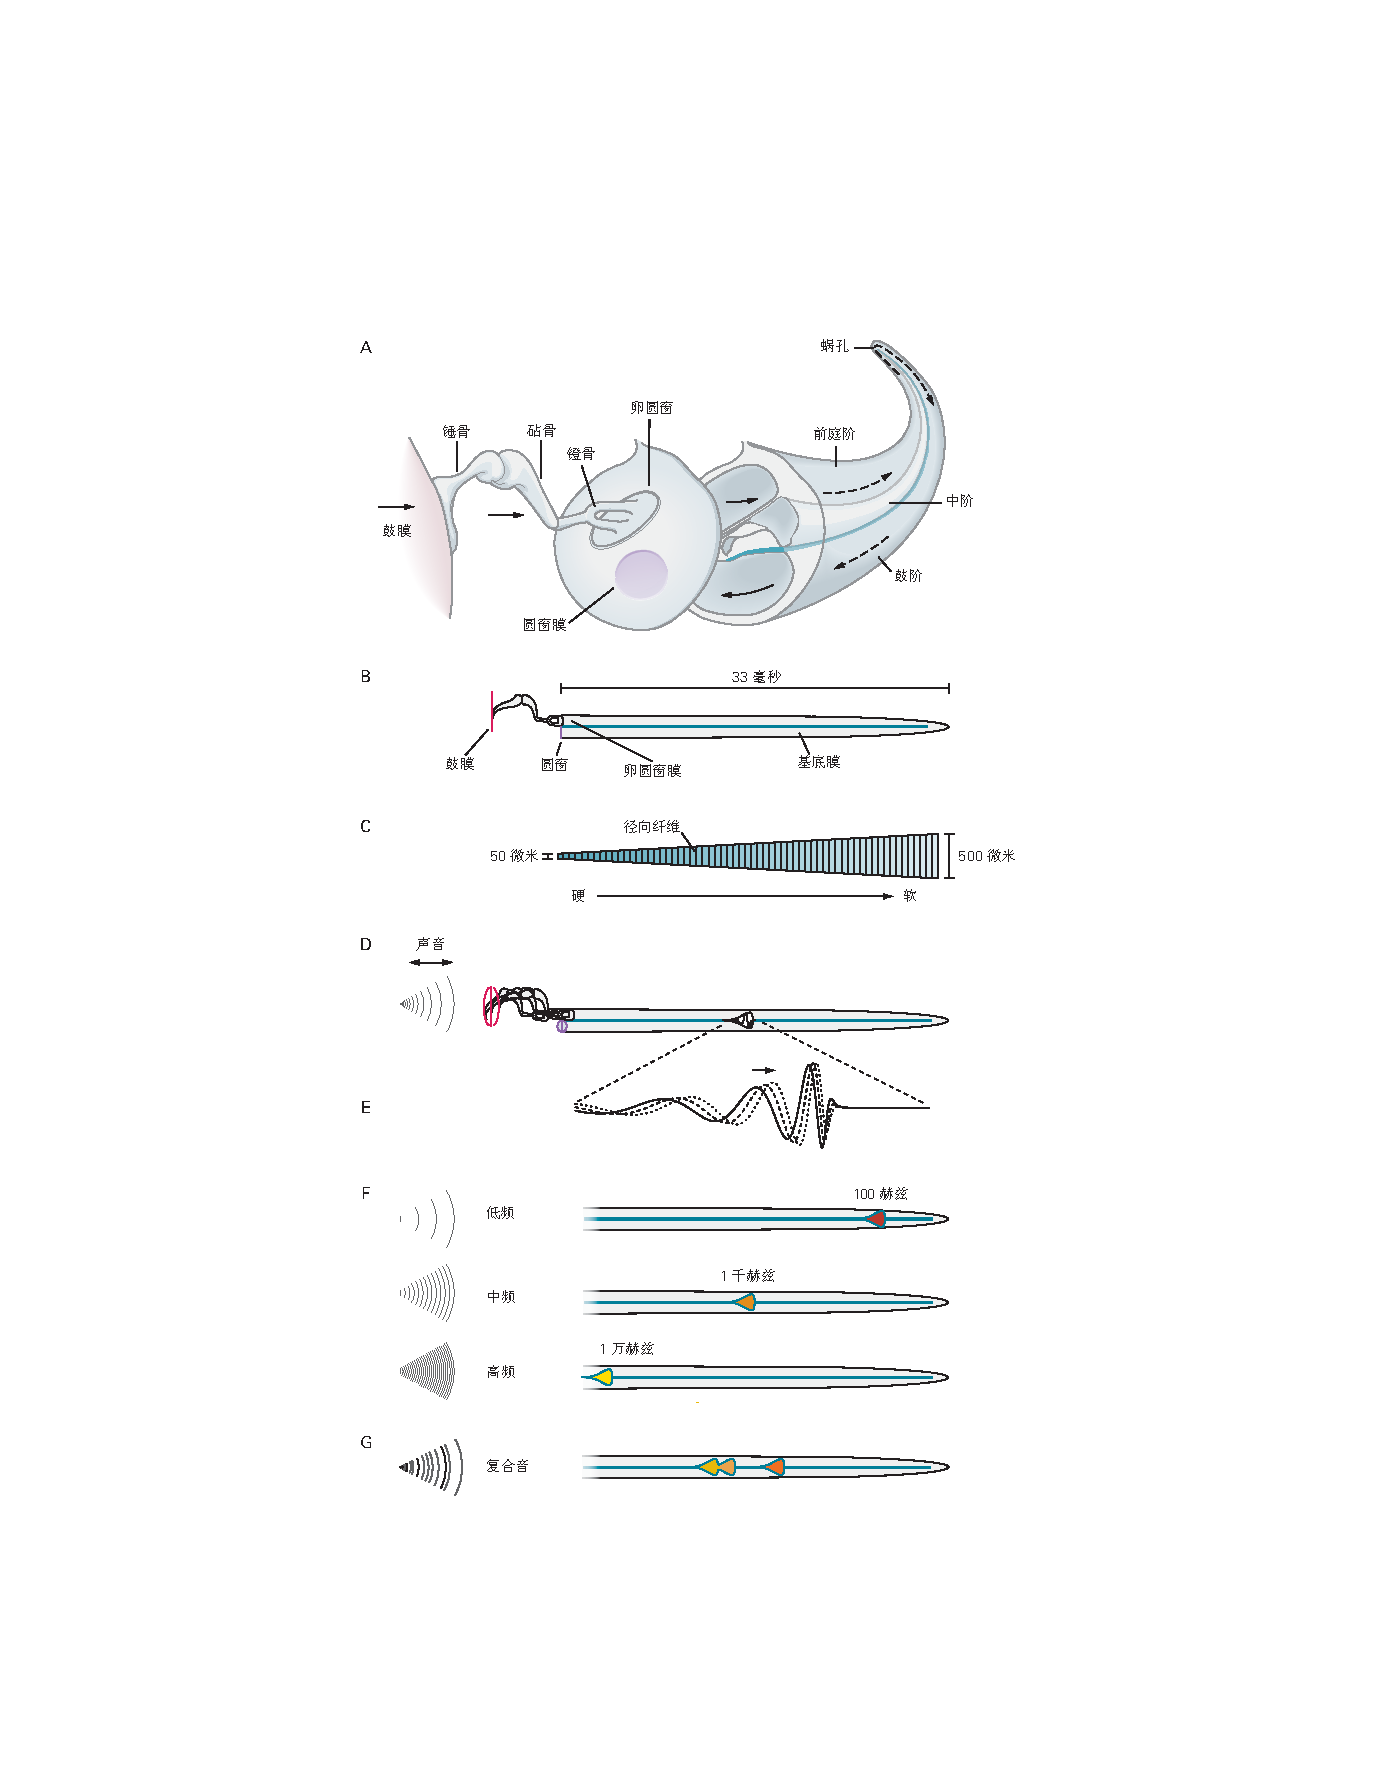
\includegraphics[width=0.5\linewidth]{chap26/fig_26_3}
	\caption{(相反)基底膜的运动。 
		A. 展开的耳蜗,其基部移位以显示其与阶梯的关系,表明刺激能量的流动。 
		声音使鼓膜振动,从而使中耳的三个听小骨运动。 
		镫骨的活塞状作用,部分插入弹性椭圆窗的骨头,产生振荡压力差,沿着前庭阶和鼓阶快速传播。 低频压力差通过 helicotrema 分流,两个管道在这里相通。 
		B. 如果耳蜗被视为线性结构,只有两个由弹性基底膜隔开的充满液体的隔室,则耳蜗的功能特性在概念上得到简化。 
		C. 此处以表面视图表示的基底膜宽度从基部附近的约 50 μm 增加到耳蜗顶端附近的 500 μm。 
		径向胶原纤维从神经到膜的神经外边缘。 由于其形态梯度,基底膜的机械性能沿其长度连续变化。 
		D. 声音的振荡刺激在基底膜上引起行波,此处显示在整个周期内的最大位移范围内。 
		运动幅度在垂直方向上被严重夸大了; 可容忍的最大声音仅使基底膜移动±150 nm,比例距离小于这些图中代表基底膜的线条宽度的百分之一。
		E. D 中活动区域的扩大表明基底膜响应单频声音刺激的运动。 连续曲线描绘了一个瞬间的行波; 基底膜偏转的垂直尺度被夸大了大约一百万倍。 虚线和虚线曲线描绘了行波在从耳蜗底部(左)向顶点(右)前进时的连续时间。 当波接近刺激频率的特征位置时,它会减慢并增加振幅。 然后刺激能量被转移到波峰内位置的毛细胞。 
		F. 每个刺激频率都会在基底膜的特定位置激发最大运动。 低频声音会在顶点附近产生基底膜运动,此处的基底膜相对较宽且柔软。 中频声音会激发中间的膜。 我们能听到的最高频率在其狭窄、僵硬的底部激发基底膜。 声频在基底膜上的映射大致呈对数关系。 
		G. 基底膜对复杂的声音进行频谱分析。 在此示例中,具有三个显着频率的声音(例如元音的三个共振峰)会激发三个区域的基底膜运动,每个区域代表一个特定的频率。 相应位置的毛细胞将基底膜振荡转化为受体电位,进而激发支配这些特定区域的神经纤维。}
	\label{fig:26_3}
\end{figure}


镫骨的作用产生压力变化,压力变化以水中的声速传播通过前庭阶的液体。 
然而,因为液体实际上是不可压缩的,所以镫骨运动的主要作用是在一个不受刚性边界限制的方向上移动前庭阶中的液体:朝向弹性耳蜗分区(图\ref{fig:26_3}B)。 
耳蜗隔板的向下偏转增加了鼓阶中的压力,取代了导致圆窗向外弯曲的液体物质。 
因此,声音刺激的每个周期都会在耳蜗的三个腔室中的每一个腔室中引起微小体积液体的上下运动循环,从而取代感觉器官。


通过将压力变化的幅度增加多达 30 倍,中耳的整体效果是将耳外空气的低阻抗与耳蜗隔板的较高阻抗相匹配,从而确保声能的高效传递 从第一种媒介到第二种媒介。 
中耳所提供的压力增益取决于声音的频率,决定了听阈的U型调谐曲线。


中耳正常结构的变化会降低其位移幅度,从而导致传导性听力损失,其中两种形式尤为常见。 
首先,由中耳感染(中耳炎)引起的疤痕组织可以固定鼓膜或听小骨。 
其次,听小骨韧带附着处的骨质增生会降低其正常的活动自由度。 
这种来源不明的慢性疾病称为耳硬化症,可导致严重的耳聋。


临床医生可以通过简单的林纳试验来测试传导性听力损失。 
要求患者在两种情况下评估振动音叉的响度:当音叉悬在空中时或当它紧靠耳朵后面的头部时。 
对于第二个刺激,声音通过骨骼传导到耳蜗。 
如果感知到第二个刺激声较大,则患者通过中耳的传导通路可能受损,但内耳很可能完好无损。 
相反,如果骨传导不比空气刺激更有效,则患者可能有内耳损伤,即感音神经性听力损失。 
传导性听力损失的诊断很重要,因为手术干预非常有效:去除疤痕组织或用假体重建传导通路可以恢复出色的听力。


\section{耳蜗的流体动力学和机械装置向受体细胞提供机械刺激}

\subsection{基底膜是声频的机械分析仪}
基底膜的机械性能沿耳蜗长度(大约 33 毫米)的连续变化是耳蜗运行的关键。 
人类耳蜗底部的基底膜宽度不到顶部的五分之一。 
因此,虽然耳蜗腔从器官的底部向其顶端逐渐变小,但基底膜的宽度却增加了(图\ref{fig:26_3}C)。 
此外,基底膜在耳蜗底部相对较厚,但在顶部较薄。 
两种形态学梯度都有助于基底膜刚度从基部到顶点的降低。 
膜内的径向胶原纤维决定了它的大部分弹性。 
基底膜可以示意性地被视为一组弱耦合的径向部分,其长度沿耳蜗的纵轴增加,最短的部分在底部,最长的部分在顶点,类似于钢琴的多根弦。


纯音刺激唤起基底膜复杂而优雅的运动。 
在一个音调的一个完整周期内,沿基底膜的每个受影响的部分都会经历一个振动周期(图\ref{fig:26_3}D、E)。
然而,膜的不同部分并不彼此同相振荡。 
正如 Georg von Békésy 使用频闪照明首次证明的那样,每个部分比其基本邻居稍晚达到其最大运动幅度。 
基底膜的归一化正弦运动再现了镫骨的运动,但时间延迟随着与耳蜗底部的距离而增加。

\begin{figure}[htbp]
	\centering
	\includegraphics[width=0.5\linewidth]{chap26/fig_26_4}
	\caption{Corti 人体器官的细胞结构。 尽管物种之间存在差异,但所有哺乳动物的基本计划都是相似的。 
		A. Corti 器,内耳的感受器官,是一种覆盖在弹性基底膜上的上皮带。 
		该器官包含约 16,000 个毛细胞,排列成四排:单排内毛细胞和三排外毛细胞。 
		这些受体细胞的机械敏感毛束伸入内淋巴,内淋巴中的液体。 
		Reissner 膜提供阶介质的上边界,将前庭阶中的内淋巴与外淋巴分开。 
		外毛细胞的毛束在其顶部附着在盖膜的下表面,盖膜是一个延伸至基底膜全长的凝胶状架子。 
		B. 毛细胞由柱状细胞和 Deiters 细胞分隔并支撑。 
		一个毛细胞已从中间一排外毛细胞中移除,以揭示支持细胞和毛细胞之间的三维关系。 
		传入和传出神经末梢分别以红色和绿色着色。}
	\label{fig:26_4}
\end{figure}


膜的整体运动模式是行波,从坚硬的底部向较软的顶点穿过耳蜗。 
随着每个波向顶点前进,振动的幅度增长到最大值,然后迅速下降。 
行波达到其最大振幅的位置取决于声音频率。 
耳蜗底部的基底膜对最高可听频率的反应最好——在人类中约为 20 kHz。 
在耳蜗顶端,膜对低至 20 Hz 的频率做出响应。 
中间频率沿基底膜以连续阵列表示(图\ref{fig:26_3}F)。 
19 世纪,德国生理学家 Hermann von Helmholtz 率先认识到基底膜的运作本质上与钢琴的运作相反。 
钢琴通过将无数振动的琴弦产生的纯音组合在一起,合成出复杂的声音; 相比之下,耳蜗通过在基底膜的适当部分分离成分音调来解构复杂的声音。


对于听觉范围内的任何频率,沿着基底膜有一个特征位置,在该位置振动幅度最大。 
尽管基底膜的形态梯度是该过程的关键,但声音频率分量沿耳蜗纵轴的实际分布取决于整个耳蜗分区的机械特性。
特别是,正如我们稍后将详述的那样,柯蒂氏器官内的毛细胞提供主动的机械反馈,从而加强基底膜的机械调节并增强其对声音的敏感性。 
振动频率沿基底膜的排列是音调图的一个例子。 
沿基底膜的频率和位置之间的关系单调变化,但不是线性的; 频率的对数大致与距耳蜗底部的距离成正比。 
从 20 kHz 到 2 kHz 的频率、2 kHz 到 200 Hz 之间的频率以及跨越 200 Hz 到 20 Hz 的频率分别代表基底膜范围的大约三分之一。


对复杂声音的反应分析说明了基底膜在日常生活中的运作方式。 
例如,人类语音中的元音通常包含三个主要频率分量,称为共振峰。 
刺激的每个频率分量都会建立一个行波,该行波在第一次近似时独立于其他波引起的波(图\ref{fig:26_3}G),并在基底膜上适合该频率分量的点处达到其峰值偏移。 
因此,基底膜通过将与刺激的不同频率分量相关的能量分配到沿其长度排列的毛细胞,从而充当机械频率分析器。
在这样做的过程中,基底膜开始对声音中的频率进行编码。


\subsection{科蒂氏器官是耳蜗中机电转导的部位}
Corti 器是沿基底膜延伸的上皮脊,是内耳的受体器官。 
科蒂氏器官的每个器官包含大约 16,000 个毛细胞,由大约 30,000 根传入神经纤维支配; 这些是沿着第八对脑神经将信息传送到大脑的纤维。 
与基底膜本身一样,每个毛细胞对特定频率最敏感,这些频率从耳蜗底部到顶部按降序对数映射。 
因此,由这些感觉细胞传输到其支配神经纤维的信息也是按音调组织的。


柯蒂氏器包括多种细胞,一些功能未知,但有四种类型具有明显的重要性。 
首先,有两种类型的毛细胞。 
内毛细胞形成一排大约 3,500 个细胞,而大约 12,000 个外毛细胞位于远离耳蜗螺旋中心轴的三排中(图\ref{fig:26_4})。 
内毛细胞和外毛细胞之间的空间由柱状细胞界定和机械支撑。 
外毛细胞的基部由 Deiters 的(指骨)细胞支撑。


第二个上皮脊与科蒂氏器官相邻,但更靠近耳蜗的中轴,产生盖膜,即覆盖 Corti 器的凝胶状架子(图\ref{fig:26_4})。 
盖膜固定在其底部,其锥形远端边缘与科蒂氏器官形成脆弱的连接。


毛细胞不是神经元; 它们缺乏树突和轴突(图\ref{fig:26_5}A)。 
一种特殊的盐溶液,即充满鳞状介质的内淋巴,浸润着细胞的顶端。 
毛细胞和支持细胞之间的紧密连接将这种液体与接触细胞基底外侧表面的标准细胞外液或外淋巴液分开。 
在紧密连接的正下方,桥粒连接为毛细胞与其相邻细胞提供了牢固的机械连接。


\begin{figure}[htbp]
	\centering
	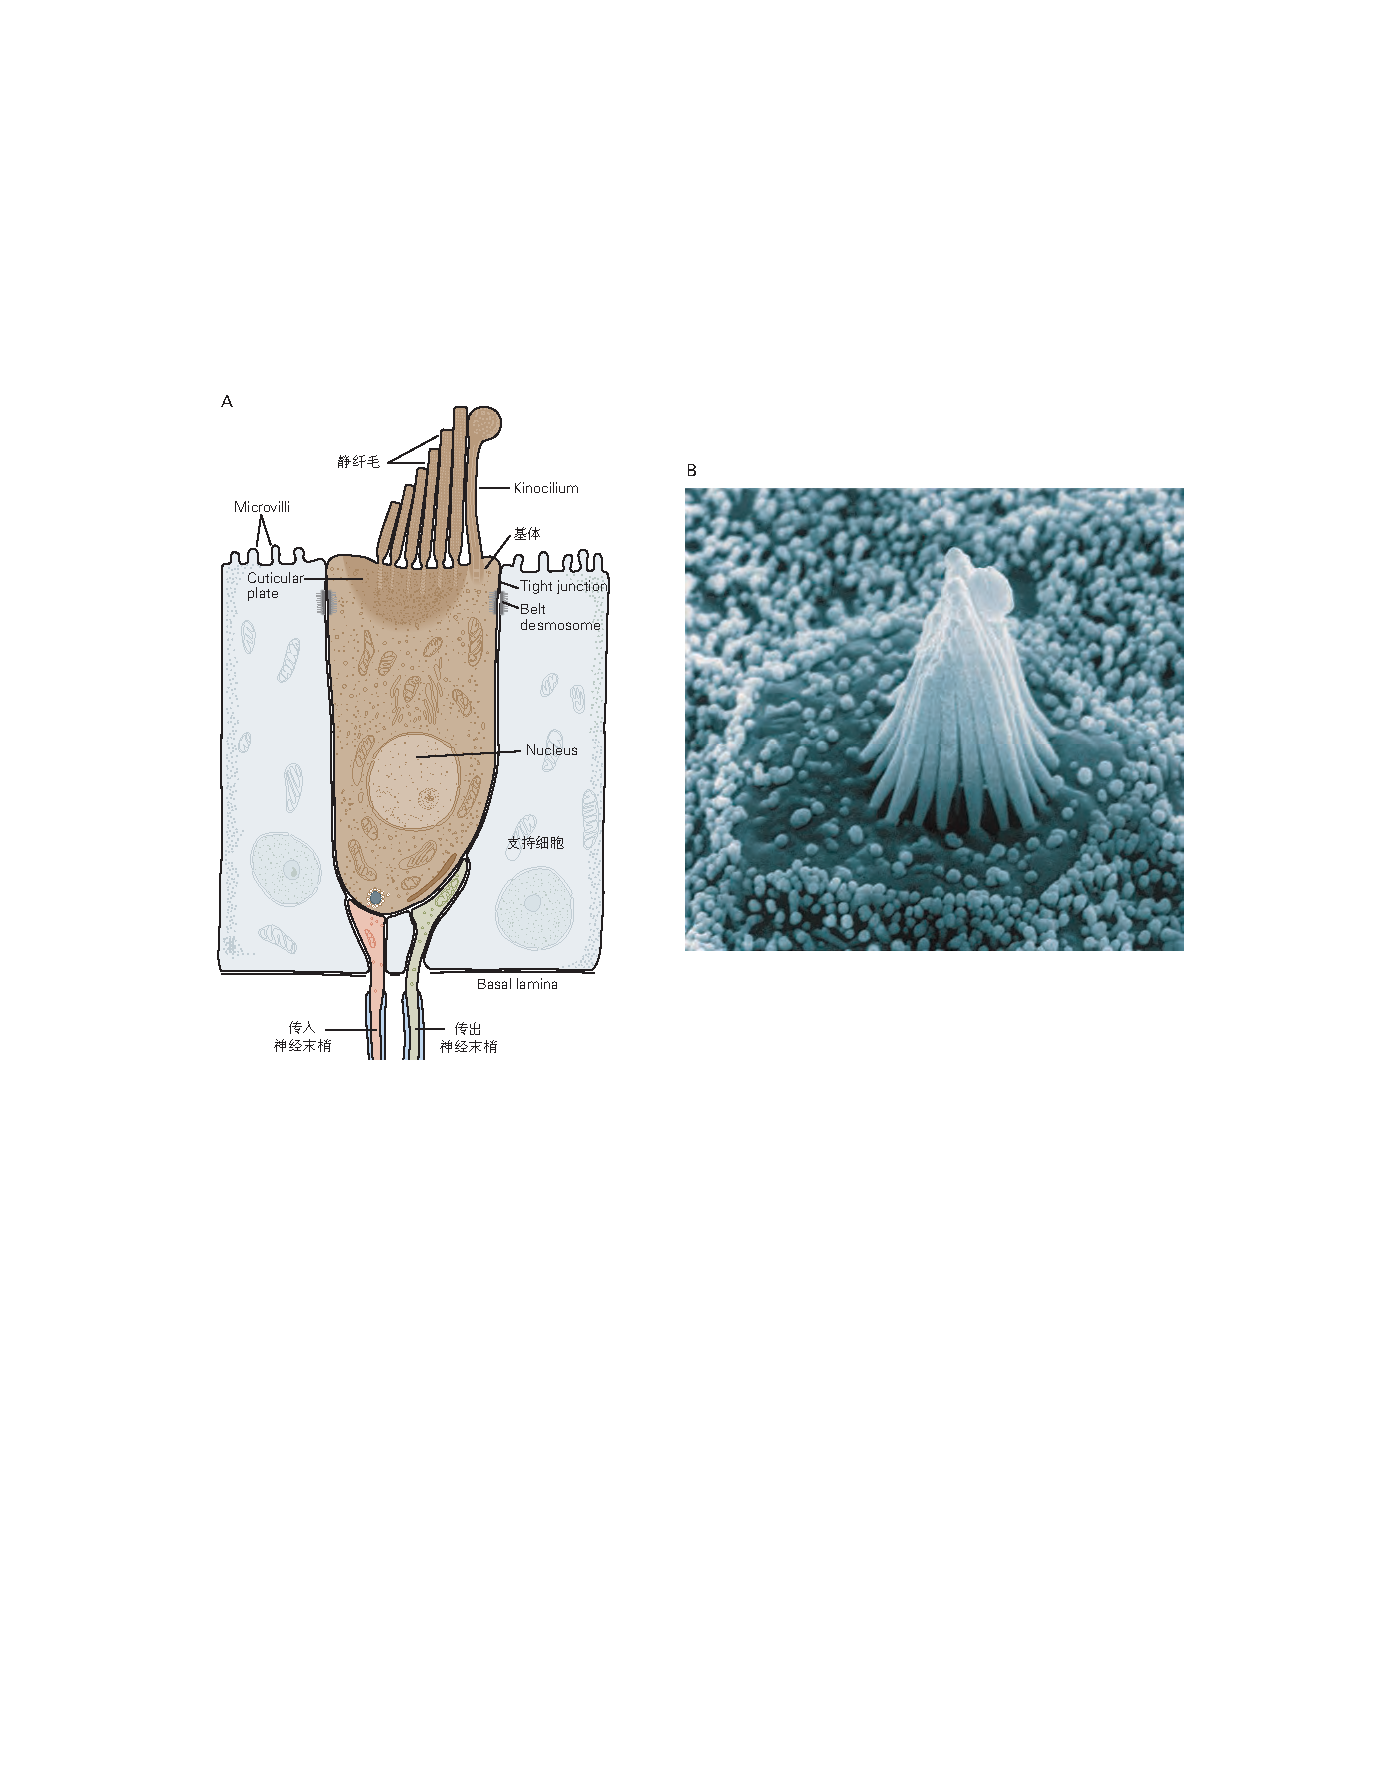
\includegraphics[width=0.5\linewidth]{chap26/fig_26_5}
	\caption{(左)脊椎动物毛细胞的结构。 
		A. 毛细胞的上皮特性在这张青蛙内耳的感觉上皮图中很明显。 
		圆柱形毛细胞通过其顶端周围的连接复合体连接到相邻的支持细胞。 
		毛束是一种机械敏感的细胞器,从细胞的顶端表面延伸出来。 
		该束包括约 60 个静纤毛,排列成不同长度的阶梯状行。 在束的高边站着单个 kinocilium,这是一种轴丝结构,其尖端有球状肿胀; 在哺乳动物的耳蜗中,这种细胞器会在出生前后退化。 毛束顶部向右偏转使毛细胞去极化; 相反方向的运动引起超极化。 毛细胞被支持细胞包围,支持细胞的顶端表面有一小撮微绒毛。 传入和传出突触接触质膜的基底外侧表面。 
		B. 这张毛细胞顶端表面的扫描电子显微照片显示,毛束突出到内淋巴中约 8 μm。 (图片经许可转载自 A.J. Hudspeth。)}
	\label{fig:26_5}
\end{figure}


毛发束作为机械刺激的接收天线,从毛细胞的扁平顶面突出。 
每个束包含几十到几百个圆柱形突起,静纤毛,排列成 2 到 10 平行行,并从细胞表面延伸几微米。 
细胞表面连续的静纤毛在高度上单调变化; 发束像皮下注射针头一样倾斜(图\ref{fig:26_5}B)。 
从上面看,哺乳动物耳蜗的内部毛细胞束大致呈线性。 
相反,外毛细胞束呈 V 形或 W 形(图 26-6)。

\begin{figure}[htbp]
	\centering
	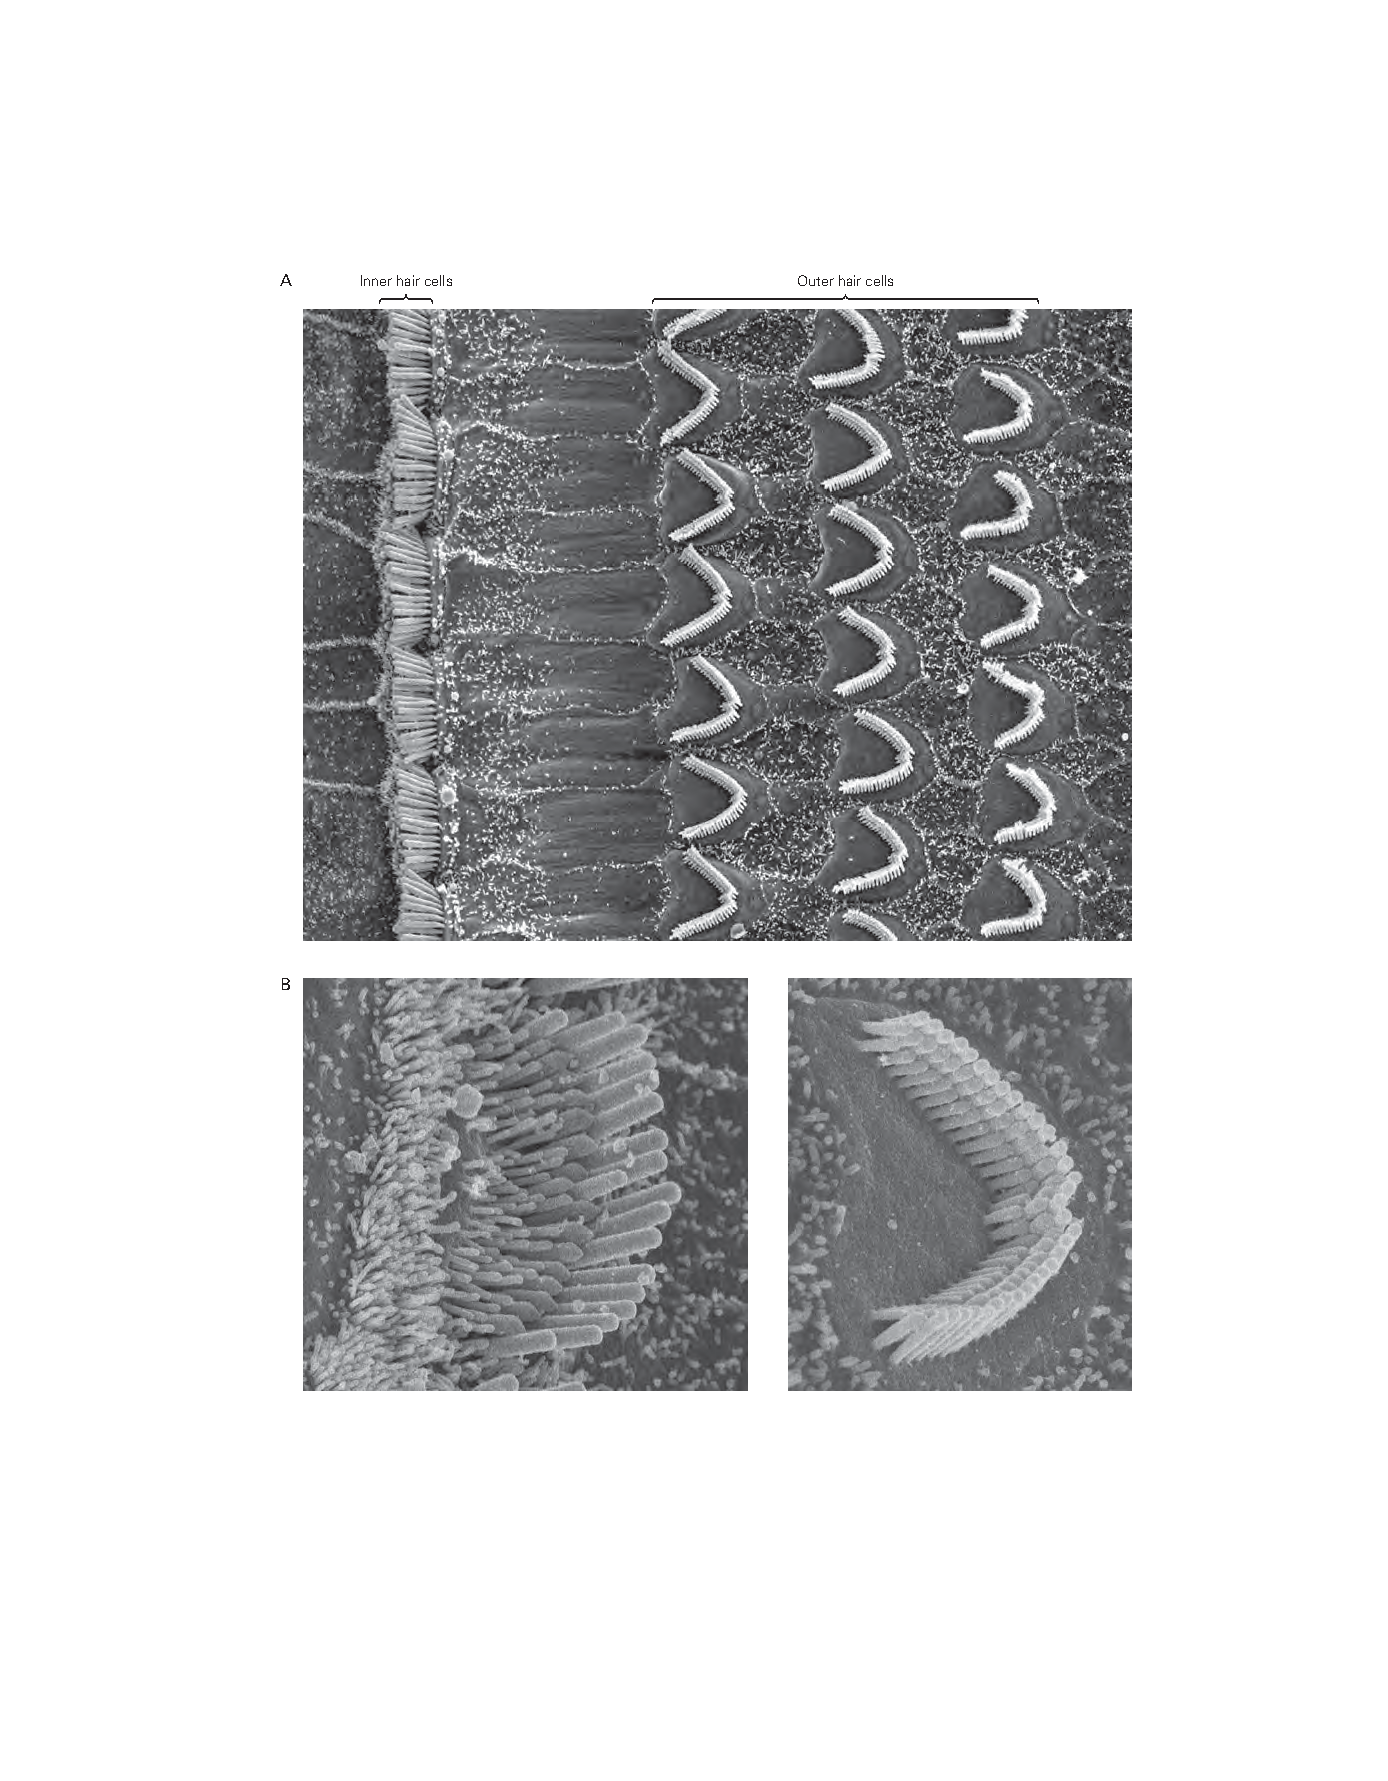
\includegraphics[width=0.5\linewidth]{chap26/fig_26_6}
	\caption{科蒂氏器官中毛细胞的排列。
		(图像经许可转载自英国基尔大学的 D. Furness。) 
		A. 内毛细胞排成一排,每个细胞的静纤毛呈直线排列。 
		相反,外毛细胞呈三排分布,每个细胞的静纤毛呈V字型排列。 
		其他几个细胞的顶面可见:从左到右,内螺旋沟细胞、柱状细胞、Deiters 细胞和 Hensen 细胞(见图 \ref{fig:26_4})。 
		B. 更高的放大倍数显示了内毛细胞顶部毛束的线性结构(左)和外毛细胞束的 V 形结构(右),以及静纤毛按高度增加的行排列。}
	\label{fig:26_6}
\end{figure}


每个静纤毛都是一个刚性圆柱体,其核心由一束肌动蛋白丝组成,这些肌动蛋白丝被塑蛋白(菌毛蛋白)、肌成束蛋白和 epsin 严重交联。 
交联使静纤毛比一束未连接的肌动蛋白丝预期的要坚硬得多。 
静纤毛的肌动蛋白核心被质膜管状鞘覆盖。 
虽然静纤毛在其大部分长度上的直径是恒定的,但它在其基底插入点上方逐渐变细(见图\ref{fig:26_5}B)。 
相应地,肌动蛋白丝的数量从几百条减少到只有几十条。 
这种薄的微丝簇将静纤毛固定在角质层板中,角质层板是顶端细胞膜下方相互连接的肌动蛋白丝的厚网。 
由于这种锥形结构,在尖端施加的机械力会导致静纤毛围绕其基底插入点旋转。 
水平顶部连接器在其尖端附近互连相邻的静纤毛。 
这些细胞外丝限制束在低频刺激期间作为一个单元移动。 
在高频下,静纤毛之间液体的粘度也反对它们的分离,从而确保毛束的单一运动。


在其早期发育过程中,每个毛束在其高边都包含一根真正的纤毛,即 kinocilium(图\ref{fig:26_5})。 
与其他纤毛一样,这种结构的核心有一个轴丝,或九对微管阵列,通常还有一对额外的中央微管。 
kinocilium 对于机械电转导不是必不可少的,因为在哺乳动物的耳蜗毛细胞中,它会在出生时退化。


\section{毛细胞将机械能转化为神经信号}


\subsection{发束的偏转引发机电转导}
正如前庭器官(第 \ref{chap:chap27} 章)一样,发束的机械偏转是刺激耳蜗毛细胞的刺激物。 
刺激通过打开或关闭(称为“门控”的过程)机械敏感离子通道引发电反应,即受体电位。 
毛细胞的反应取决于刺激的方向和强度。


在未受刺激的细胞中,参与刺激转导的通道中有 10\% 至 50\% 是开放的。 
因此,位于大约 –70 至 –30 mV 范围内的细胞静息电位部分取决于通过这些通道流入的阳离子。 
将束移向其高边的刺激会打开额外的通道,从而使细胞去极化(图 26-7)。 
相比之下,将束移向其短边的刺激会关闭静止时打开的转导通道,从而使细胞超极化。 
毛细胞对平行于毛束形态镜像对称轴的刺激反应最大:与轴成直角的刺激与静息电位相比几乎没有变化。 
倾斜刺激引起与其沿灵敏度轴的矢量投影成比例的响应。

\begin{figure}[htbp]
	\centering
	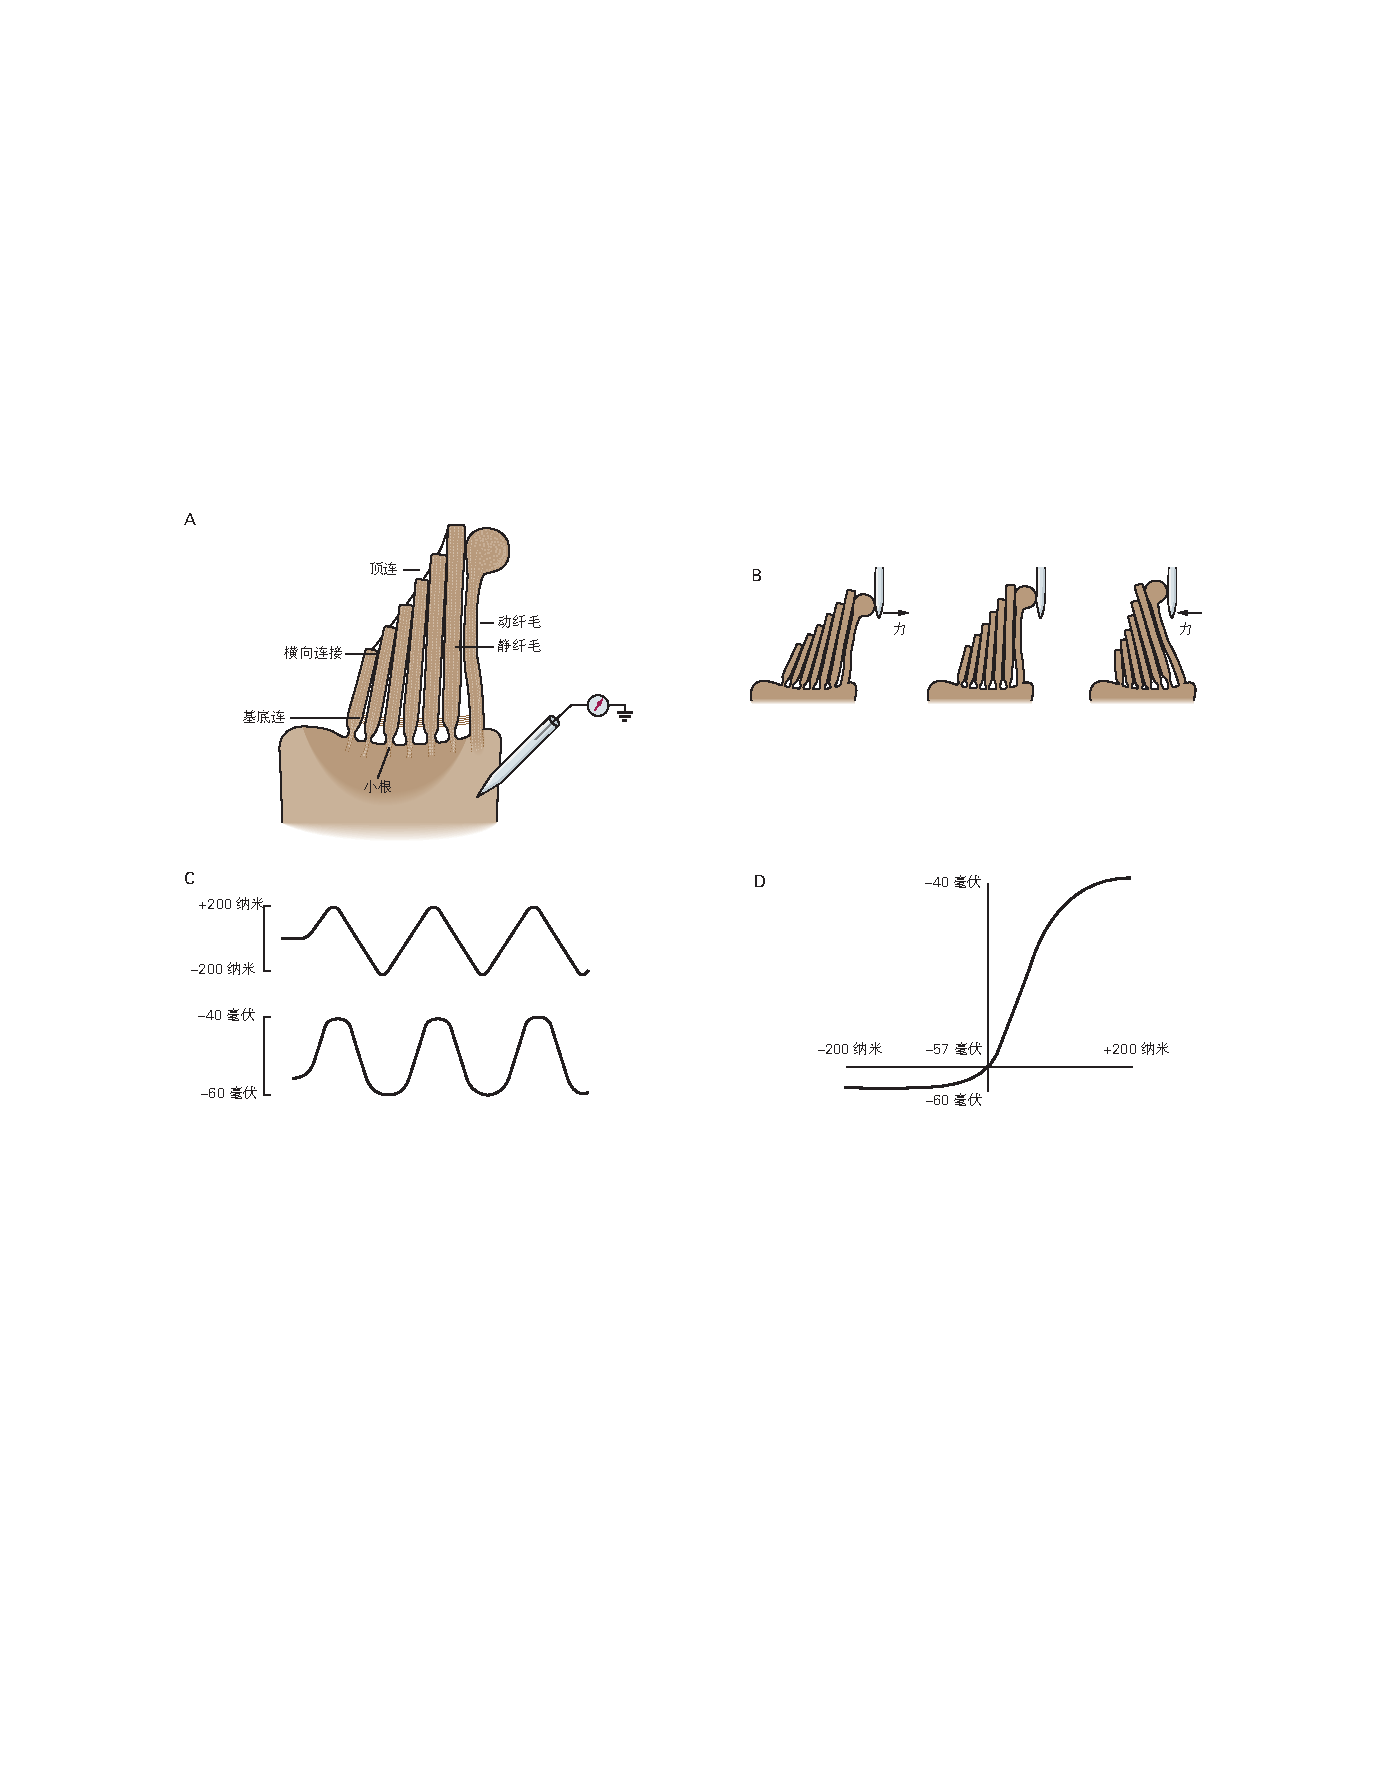
\includegraphics[width=0.5\linewidth]{chap26/fig_26_7}
	\caption{(左)毛细胞的机械敏感性。 
		A. 记录电极插入蛙毛细胞。 
		B. 连接到静纤毛球状尖端的探针由压电刺激器移动,使弹性发束从其静止位置偏转。 
		实际偏转通常只有所描绘的偏转的十分之一。 
		C. 当发束的顶部来回移动时(上部迹线),机械敏感离子通道的打开和关闭会产生振荡受体电位(下部迹线)——如此处——可能在去极化和去极化中饱和 超极化方向。 
		D. 发束偏转(横坐标)和受体电位(纵坐标)之间的关系是 S 形的。 
		整个操作范围只有大约 100 nm,小于单个静纤毛的直径。 
		静止时,发束在 S 状结肠的陡峭区域内运行,这确保了对微弱刺激的反应具有显着的受体电位。}
	\label{fig:26_7}
\end{figure}


毛细胞的受体电位是分级的。 
随着刺激幅度的增加,受体电位逐渐增大直至达到饱和点。 
内毛细胞的受体电位峰峰值幅度可高达 25 mV。 
束的偏转和产生的电响应之间的关系是 S 形的(图 26-7D)。 
仅 ±100 nm 的位移代表大约 90\% 的响应范围。 
在正常刺激过程中,一束发束以±1°左右的角度移动,即远小于一个静纤毛的直径。


在体外观察时,发束表现出大约 ±3 nm 的布朗运动,而听觉阈值对应于低至 ±0.3 nm 的基底膜运动。 
至少有三种机制可以解释发束如何响应小于其自身噪音的运动。 
首先,由于耳蜗隔板不作为刚体运动,因此毛束的运动大于基底膜的运动。 
其次,低刺激的频率选择性放大主动将信号从噪声中拉出。 
最后,与一组邻居的机械耦合导致有效降低噪声的同步。 
在听力阈值处,刺激会引起振幅接近 100 μV 的受体电位。


毛细胞中介导机械电转导的离子通道是相对非选择性的阳离子传递孔,电导接近 100 pS。 
从已知大小的可以穿过通道的有机小阳离子和荧光分子来看,转导通道的孔径必须在 1.3 nm 左右。 
大部分转导电流由 K+ 携带,K+ 是沐浴毛束的内淋巴中浓度最高的阳离子。 
尽管内淋巴中的 Ca2+ 相对较少,但该离子携带了一小部分转导电流。 
荧光指示剂表明 Ca2+ 进入,因此机械电转导,恰好发生在偏转发束的立体纤毛尖端。 
单通道记录,连同转导电流的大小大致与显微解剖束中剩余的功能性静纤毛数量成正比的观察结果表明,每个静纤毛可能只有两个活跃的转导通道。


孔的大直径和差的选择性允许转导通道被链霉素、庆大霉素和妥布霉素等氨基糖苷类抗生素阻断。 
当大剂量用于对抗细菌感染时,这些药物会对毛细胞产生毒性作用; 抗生素会破坏毛束并最终杀死毛细胞。 
这些药物以低速率通过转导通道,因此通过干扰类似于细菌核糖体的线粒体核糖体上的蛋白质合成而引起长期毒性作用。 
与这一假设一致,人类对氨基糖苷类药物的敏感性是母系遗传的,线粒体也是如此,并且在许多情况下反映了线粒体 12S 核糖体 RNA 基因的单个碱基变化。


\subsection{机械力直接打开转导通道}
毛细胞中转导通道的门控机制与神经元中用于电信号(例如动作电位或突触后电位)的机制根本不同。 
许多离子通道对膜电位的变化或特定配体有反应(第 \ref{chap:chap8}、\ref{chap:chap10} 和 \ref{chap:chap12}-\ref{chap:chap14} 章)。 
相反,两条证据表明毛细胞中的机械电转导通道被机械应变激活。


首先,束沿其机械灵敏度轴比直角更硬。 
这一观察表明,使束偏转的部分功进入了弹性元件,称为门控弹簧,它拉动转导通道的分子门。 
由于门控弹簧贡献了超过一半的发束刚度,因此转换通道有效地捕获了发束偏转时提供的能量。 
此外,毛束的机械特性在通道选通过程中会发生变化:当通道打开或关闭时,刚度会降低,摩擦力会增加。 
如果通道直接通过与发束的机械连接进行门控,则这两种现象都是预期的。


转导通道直接由门控弹簧控制的第二个迹象是毛细胞响应的速度。 
响应延迟非常短,只有几微秒,门控很可能是直接的,而不是涉及第二个信使(第 \ref{chap:chap14} 章)。
此外,毛细胞对一系列幅度不断增加的阶跃刺激的电响应变得更大更快。 
这种行为有利于机械力控制通道门控速率常数的动力学方案。


尖端连杆可能是门控弹簧的组成部分。 
尖端连接是一种精细的分子编织物,将一个静纤毛的远端连接到最长的相邻过程的一侧(图\ref{fig:26_8}A)。 
发束向其高边的偏转会拉紧尖端连接并促进通道打开; 相反方向的运动会松弛链接并允许相关联的通道关闭(图 \ref{fig:26_8}B)。


\begin{figure}[htbp]
	\centering
	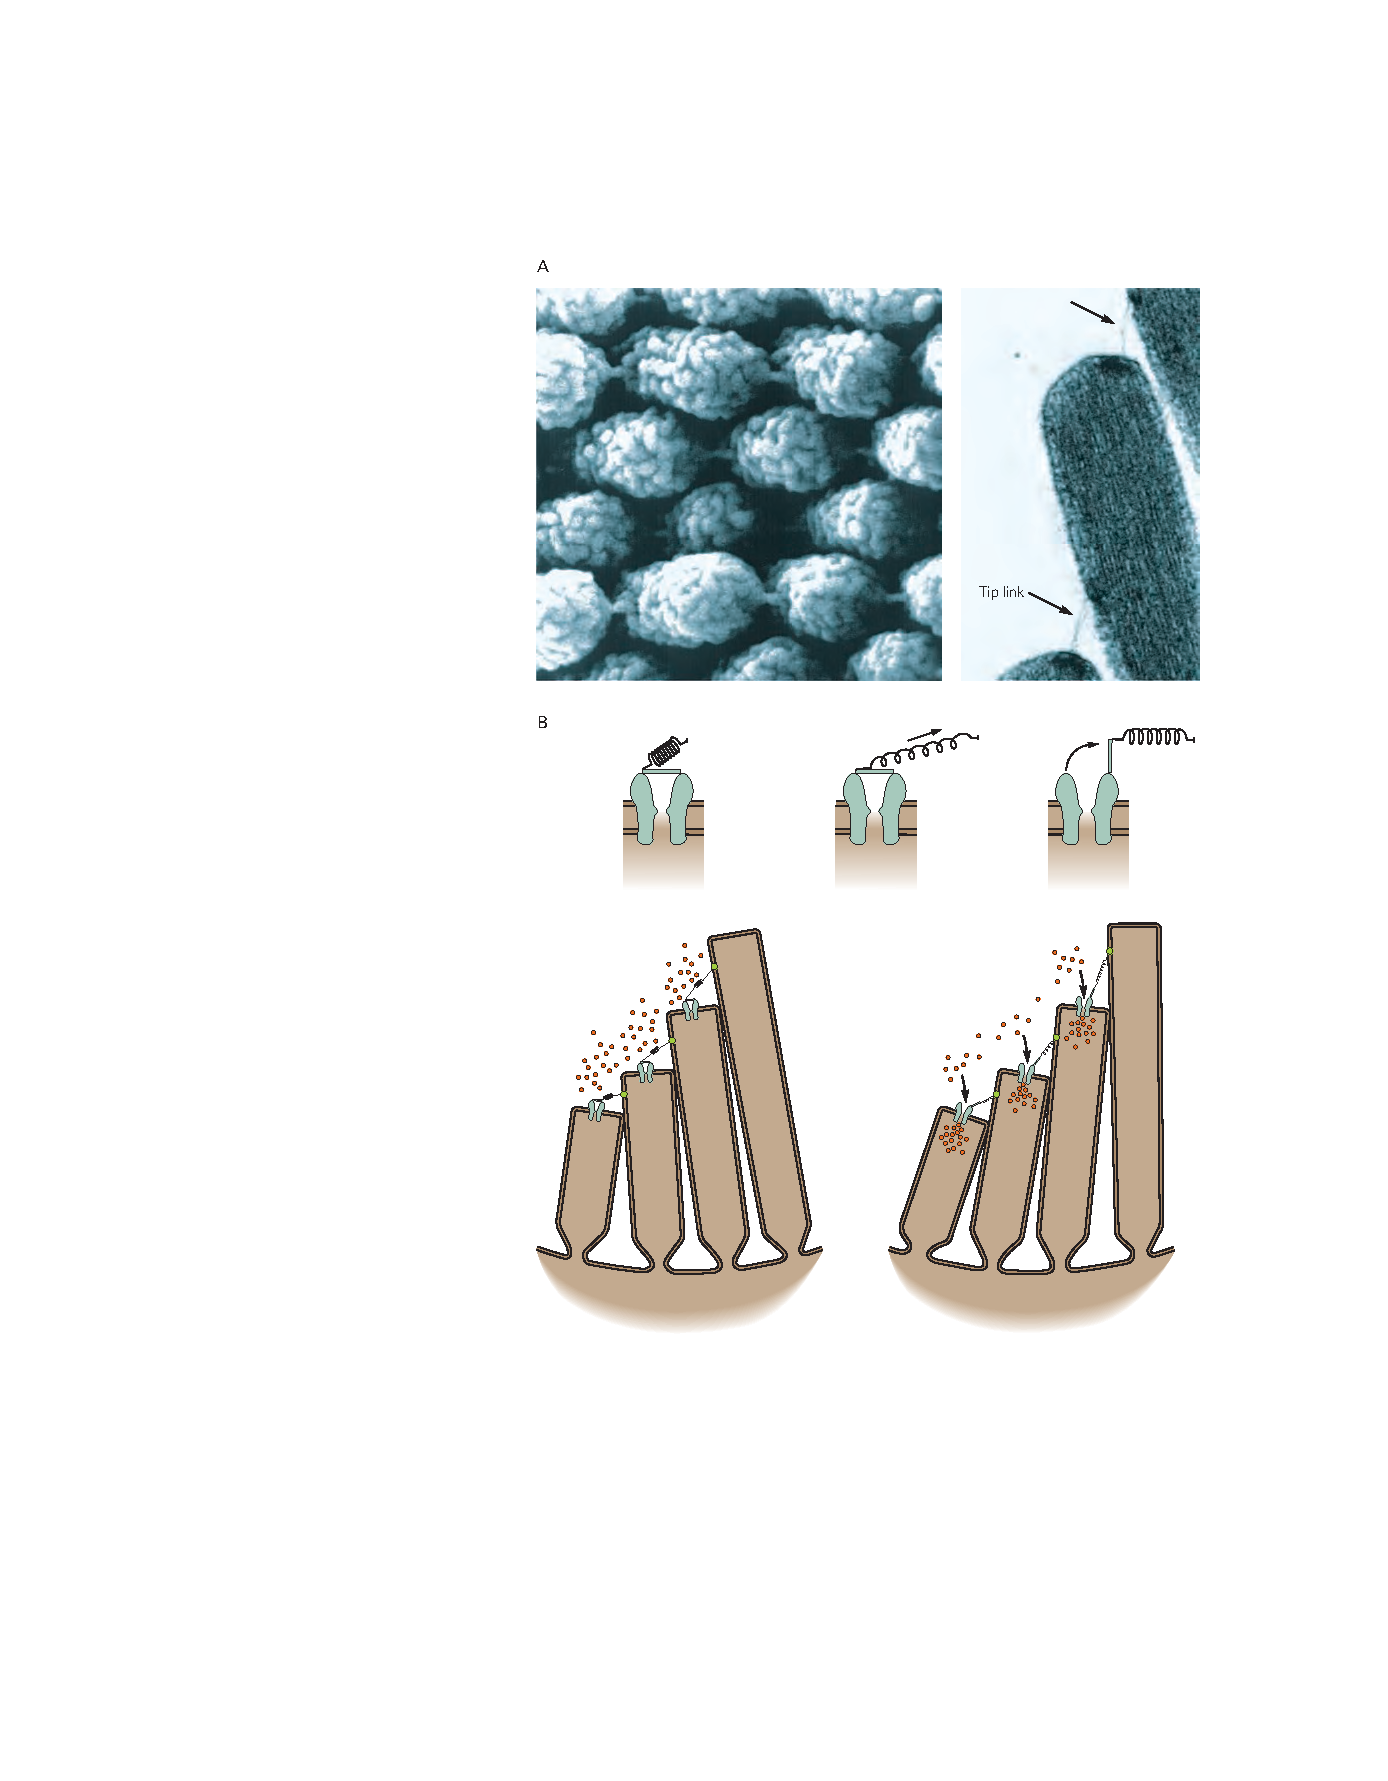
\includegraphics[width=0.5\linewidth]{chap26/fig_26_8}
	\caption{毛细胞的机械电转导。 
		A. 尖端连接将每个静纤毛连接到最长的相邻静纤毛的一侧,如发束顶面的扫描电子显微照片(左)和透射电子显微照片(右)所示。 
		每个尖端链接的直径仅为 3 nm,长度为 150 至 200 nm。 
		由于试样制备过程中的金属涂层,链接在左侧的插图中显得更坚固。 
		(经许可转载自 Assad、Shepherd 和 Corey 1991;经许可转载自 Hudspeth 和 Gillespie 1994。) 
		B. 上图:通过毛细胞中机械电转导基础通道的离子通量受分子门调节。 
		闸门的打开和关闭由弹性元件(门控弹簧)中的张力控制,门控弹簧感应发束位移。 (经许可改编自 Howard 和 Hudspeth 1988。)底部:当发束静止时,每个转导通道在关闭和打开状态之间波动,大部分时间都处于关闭状态。 
		束在正方向上的位移增加了门控弹簧的张力,这里假设部分是尖端链接,连接到每个通道的分子门。 
		增强的张力促进通道开放和阳离子流入,从而产生去极化受体电位。
		 (经许可改编自 Hudspeth 1989。)}
	\label{fig:26_8}
\end{figure}


三个实验结果表明,尖端连杆是门控弹簧的组成部分。 
首先,尖端连接是发束的普遍特征,位于转导部位。 
转导通道确实位于立体纤毛尖端,因此靠近尖端连接的下插入点。 
其次,链接的方向与转导的矢量灵敏度一致。 
这些链接总是在平行于发束的机械敏感性轴的方向上互连静纤毛。 
最后,当通过将毛细胞暴露于 Ca2+ 螯合剂而破坏尖端连接时,转导消失。 
随着尖端连接在大约 12 小时的过程中再生,毛细胞恢复了机械敏感性。 
目前还不清楚门控弹簧的弹性是主要存在于尖端连接处还是存在于它们的两个插入处的结构中。


在哺乳动物的耳蜗中,毛束通过它们与盖膜的连接而偏转。 
当基底膜响应声音上下振动时,柯蒂氏器和覆盖在其上的盖膜随之移动。 
然而,由于基底膜和盖膜围绕不同的插入线旋转,因此它们的上下运动伴随着柯蒂氏器上表面和盖膜下表面之间的来回剪切运动。 
这是由毛细胞检测到的运动(图\ref{fig:26_9})。

\begin{figure}[htbp]
	\centering
	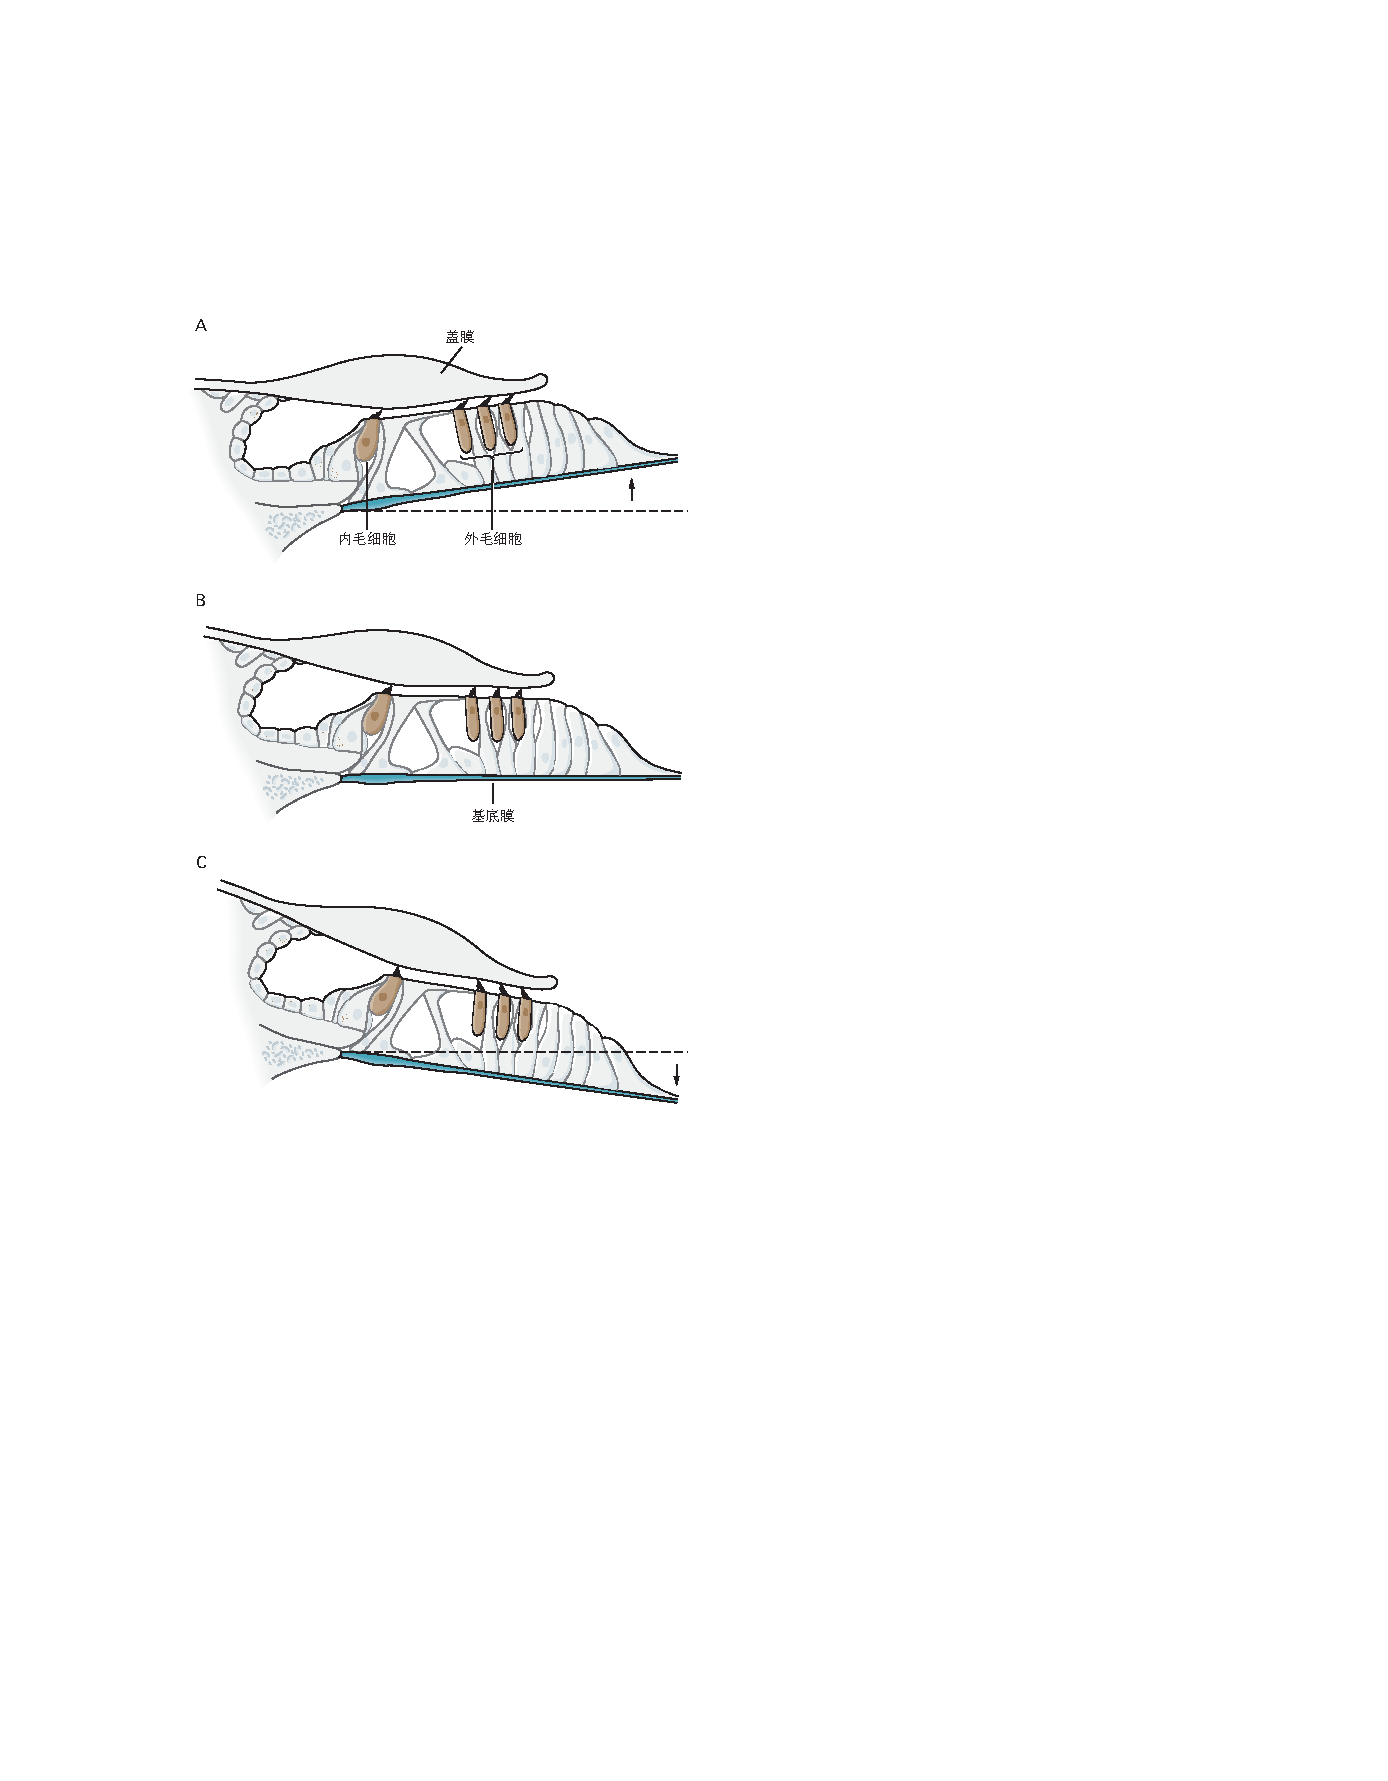
\includegraphics[width=0.5\linewidth]{chap26/fig_26_9}
	\caption{作用于耳蜗毛细胞的力。 
		当基底膜因前庭阶和鼓阶之间的压力差异而上下移动时,耳蜗中的毛细胞会受到刺激。 
		这种运动伴随着盖膜和 Corti 器官之间的剪切运动。 
		这些运动使附着在盖膜下表面的外毛细胞的毛束偏转。 
		未附着在盖膜上的内毛细胞的毛束会因该结构下方空间中液体的运动而偏转。 
		在这两种情况下,偏转都会启动刺激的机械电转换。 
		A. 当基底膜被向上驱动时,毛细胞和盖膜之间的剪切力使毛束在兴奋方向偏转,朝向它们的高边。 
		B. 在振荡的中点,发束恢复到它们的静止位置。 
		C. 当基底膜向下移动时,发束被驱动到抑制方向。}
	\label{fig:26_9}
\end{figure}


外毛细胞的毛束,其尖端牢固地附着在盖膜上,直接被这种运动偏转。 
不接触盖膜的内毛细胞的毛束会因膜下液体的运动而偏转。 
这种刺激模式为到达发束的信号提供了一些机械放大。 
至少对于高频刺激,发束的运动被认为比基底膜的运动大几倍。

\subsection{直接机电转换速度很快}
毛细胞比脊椎动物神经系统的其他感觉受体细胞运作得更快,实际上比神经元本身更快。 
为了处理生物相关声音的频率,毛细胞的转导必须快速。 
鉴于声音在空气中的行为以及发声和吸声器官(如声带和耳膜)的尺寸,最佳听觉交流发生在 10 Hz 至 100 kHz 的频率范围内。 
更高的频率在空气中传播效果差; 中等大小的动物无法有效地产生和捕获低得多的频率。 
即使在对相对较低频率敏感的动物(如青蛙)中,响应中等强度阶跃刺激的体外转导电流在室温下以仅 80 μs 的时间常数上升。 
对于能够响应大于 100 kHz 的频率的哺乳动物,毛细胞显然显示出更小一个数量级的门控时间。 
定位声源是听力最重要的功能之一,它对传导速度设置了更严格的限制(第 \ref{chap:chap28} 章)。 
从声源直接传到人一侧的声音到达较近的耳朵比到达较远的耳朵要快一些,在人类中最多 700 微秒。 观察者可以根据更小的延迟(大约 10 微秒)来定位声源。 
为此,毛细胞必须能够以微秒级分辨率转换声波波形。


\subsection{耳聋基因提供了机械传导机制的组成部分}
人类和小鼠模型中耳聋的遗传研究为了解毛细胞机械传导机制的分子组成提供了切入点。 
特别是,尖端连接的上三分之二由两个平行的 cadherin-23 分子组成,而下三分之一由两个平行的 protocadherin-15 分子组成(图 \ref{fig:26_10})。 
这两个组件以对 Ca2+ 敏感的方式在其尖端连接; 将细胞外 Ca2+ 浓度降低到大约 1 μM 以下会破坏它们的结合。 
在人类中,编码钙粘蛋白 23 (USH1D) 和原钙粘蛋白 15 (USH1F) 的基因突变会导致最严重的 Usher 综合征,这是一种常染色体隐性遗传病,与严重至极重度的先天性耳聋、持续性前庭功能障碍和 青春期前发病的视网膜色素变性。 
对涉及此类 Usher 综合征的其他基因的研究表明,尖端连接的上端通过一种蛋白质复合物锚定在静纤毛的肌动蛋白核心上,该蛋白质复合物包括支架蛋白 sans (USH1G) 和 harmonin (USH1C), 以及分子马达肌球蛋白 7a (USH1B)。

\begin{figure}[htbp]
	\centering
	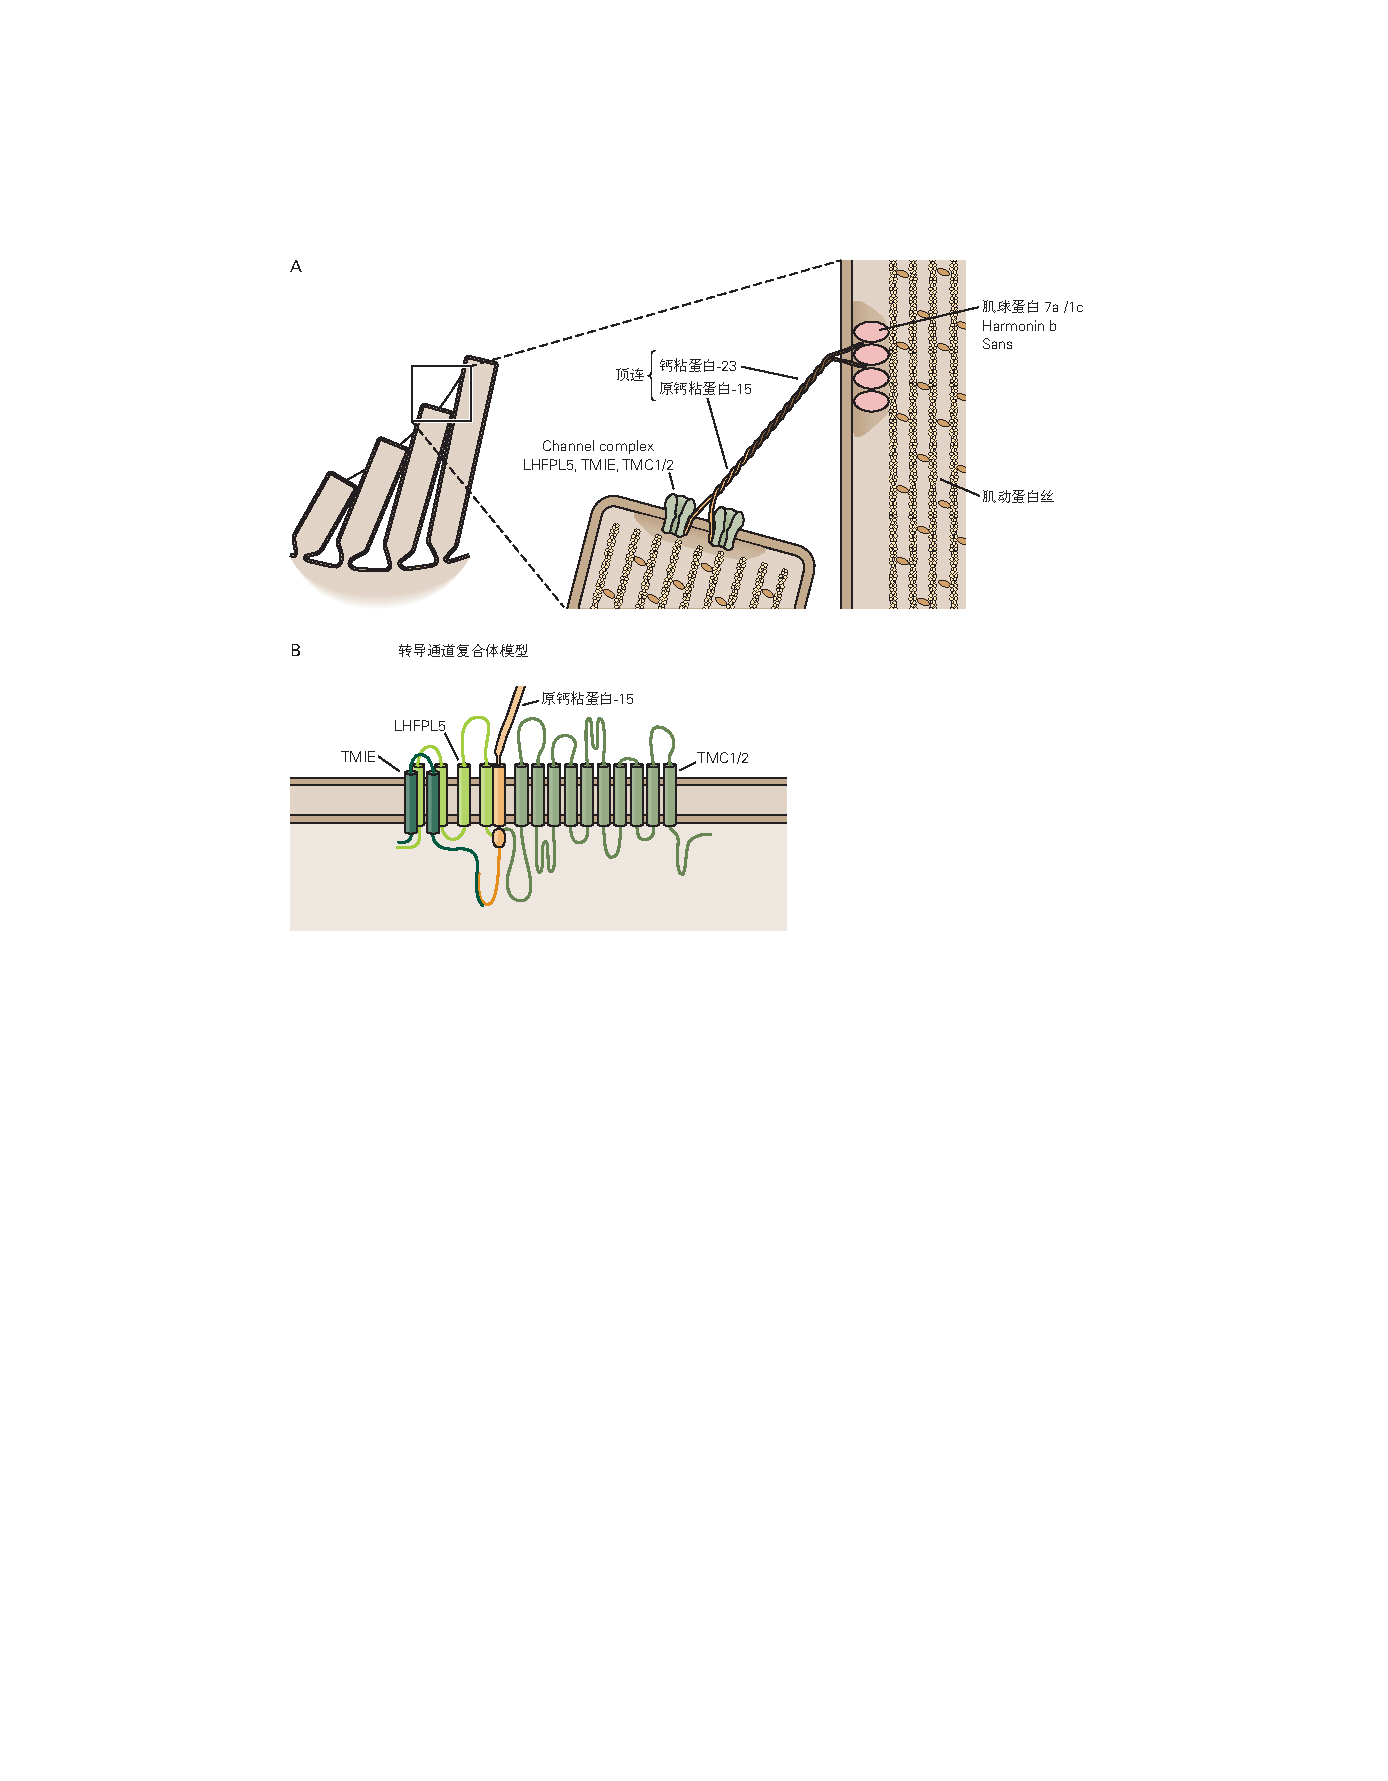
\includegraphics[width=0.7\linewidth]{chap26/fig_26_10}
	\caption{转导机制的分子组成。 A. 尖端连接由原钙粘蛋白 15 和钙粘蛋白 23 的异嗜性结合组成。两个转导通道位于较短的静纤毛尖端尖端连接的下插入点附近。 每个通道都是分子复合体的一部分,其中包括蛋白质 TMC1/2、LHFPL5 和 TMIE。 在较长静纤毛侧翼的上部插入点,钙粘蛋白 23 与协调蛋白 b 和分子马达肌球蛋白 7a 相互作用,它们都与肌动蛋白结合,从而锚定尖端连接。 蛋白质sans用作支架蛋白。 在前庭毛细胞中,肌球蛋白 1c 可能使尖端连接处于紧张状态,但这种运动蛋白在耳蜗毛细胞中的存在尚不确定。 B. 转导通道复合体模型。 TMC1/2、LHFPL5 和 TMIE 与原钙粘蛋白 15 相互作用,因此与尖端连接的下端相互作用。 TMIE 还与 LHFPL5 交互。 这些蛋白质在转导装置内的详细排列仍然未知。 与图中所示不同的是,TMC1 被提议组装成二聚体,每个 TMC1 分子都为阳离子提供渗透途径。 (经许可改编自 Wu 和 Müller 2016 以及 Pan 等人 2018。)}
	\label{fig:26_10}
\end{figure}


毛细胞中通道数量少,加上缺乏用于标记它们的高亲和力配体,解释了为什么转导通道的生化特性长期以来一直不确定。 
然而,最近的遗传、生物化学和生物物理学实验表明,四种完整的跨膜蛋白与转导通道密切相关:跨膜通道样蛋白 1 和 2(TMC1 和 TMC2)、毛细胞静纤毛中的四跨膜蛋白(TMHS;官方) 命名法 LHFPL5)和跨膜内耳表达基因(TMIE;图 \ref{fig:26_10})。 
缺乏 TMIE 的小鼠毛细胞中的机械转导被废除,即使转导机制的所有其他已知组件似乎都已正确就位。 
然而,由于 TMIE 仅包含两个预测的跨膜结构域,因此这种蛋白质单独构成离子通道的可能性很小。 
在没有 LHFPL5 的情况下,转导通道的电导降低,但仍然可以测量到显着的转导电流,表明该蛋白质不是通道孔的重要组成部分。


多条证据支持 TMC1 和 TMC2 作为转导通道的组成部分。 
这两种蛋白质都位于尖端连接的较低插入点附近,转导电流进入毛细胞,与尖端连接成分原钙粘蛋白 15 相互作用,并且它们的表达开始与机械电转导相吻合。 
此外,携带 Tmc1 基因单点突变的小鼠的转导通道显示出较低的电导率和 Ca2+ 渗透性,表明 TMC1 非常靠近通道的孔隙。 
在预计位于通道孔内或附近的位点进行的单个半胱氨酸取代证实 TMC1 属于主要传导通路。 
事实上,用带正电荷的试剂对半胱氨酸残基进行共价修饰会导致几个 TMC1 突变体的单通道电导降低。 
当发束偏向其短边(以关闭转导通道)后或通道阻滞剂阻止进入通道孔时,应用半胱氨酸修饰试剂无效。 
因此,TMC1 不太可能构成形成孔形成蛋白前庭的辅助通道亚基。 
相反,有强有力的证据表明 TMC1 至少构成了转导通道孔的一部分。 
在耳蜗毛细胞中,TMC1 和 TMC2 在新生儿发育期间共表达,但只有 TMC1 表达维持到成年期。


\section{动态反馈机制决定毛细胞的敏感性}

毛细胞必须应对能量含量非常低的声学刺激。
如果刺激由周期信号组成,例如纯音的正弦压力,则检测系统可以通过选择性地增强对相关频率的响应来增加信噪比。
毛细胞在声刺激的特征频率下反应最好。 给定毛细胞的频率选择性部分来自其机械输入的被动外在过滤,特别是哺乳动物基底膜的同位素排列的结果。 此外,当忽略低频输入是适当的时候,毛细胞拥有一种独特的适应机制,可以充当高通滤波器。 毛细胞还采用机械放大来增强和进一步调整它们的机械敏感性。

\subsection{毛细胞被调整到特定的刺激频率}
每个耳蜗毛细胞对特定频率的刺激最敏感,称为其特征频率、自然频率或最佳频率。 平均而言,相邻内毛细胞的特征频率相差约0.2\%; 相比之下,相邻的钢琴弦被调谐到相隔约 6\% 的频率。 因为即使由纯正弦刺激引起的行波也会沿着基底膜传播,所以耳蜗毛细胞的灵敏度在其特征频率上下的有限范围内延伸,刺激水平越高则越敏感。 在低水平下,纯音会募集大约 100 个毛细胞。 毛细胞的频率灵敏度可以显示为调谐曲线。 为了构建调谐曲线,实验者用低于、等于和高于细胞特征频率的许多频率的纯音刺激耳朵。 刺激水平针对每个频率进行调整,直到细胞的反应达到预定义的标准幅度。 调谐曲线是声级图,以分贝 SPL 的对数形式表示为刺激频率的函数。

内毛细胞的调谐曲线通常是 V 形的(图 \ref{fig:26_11})。 
曲线的尖端代表细胞的特征频率,即为最低刺激水平产生标准反应的频率。 更高或更低频率的声音需要更高的水平来激发细胞以达到标准反应。 由于行波的形状,调谐曲线的斜率在其高频侧翼比在低频侧翼上陡峭得多。

\begin{figure}[htbp]
	\centering
	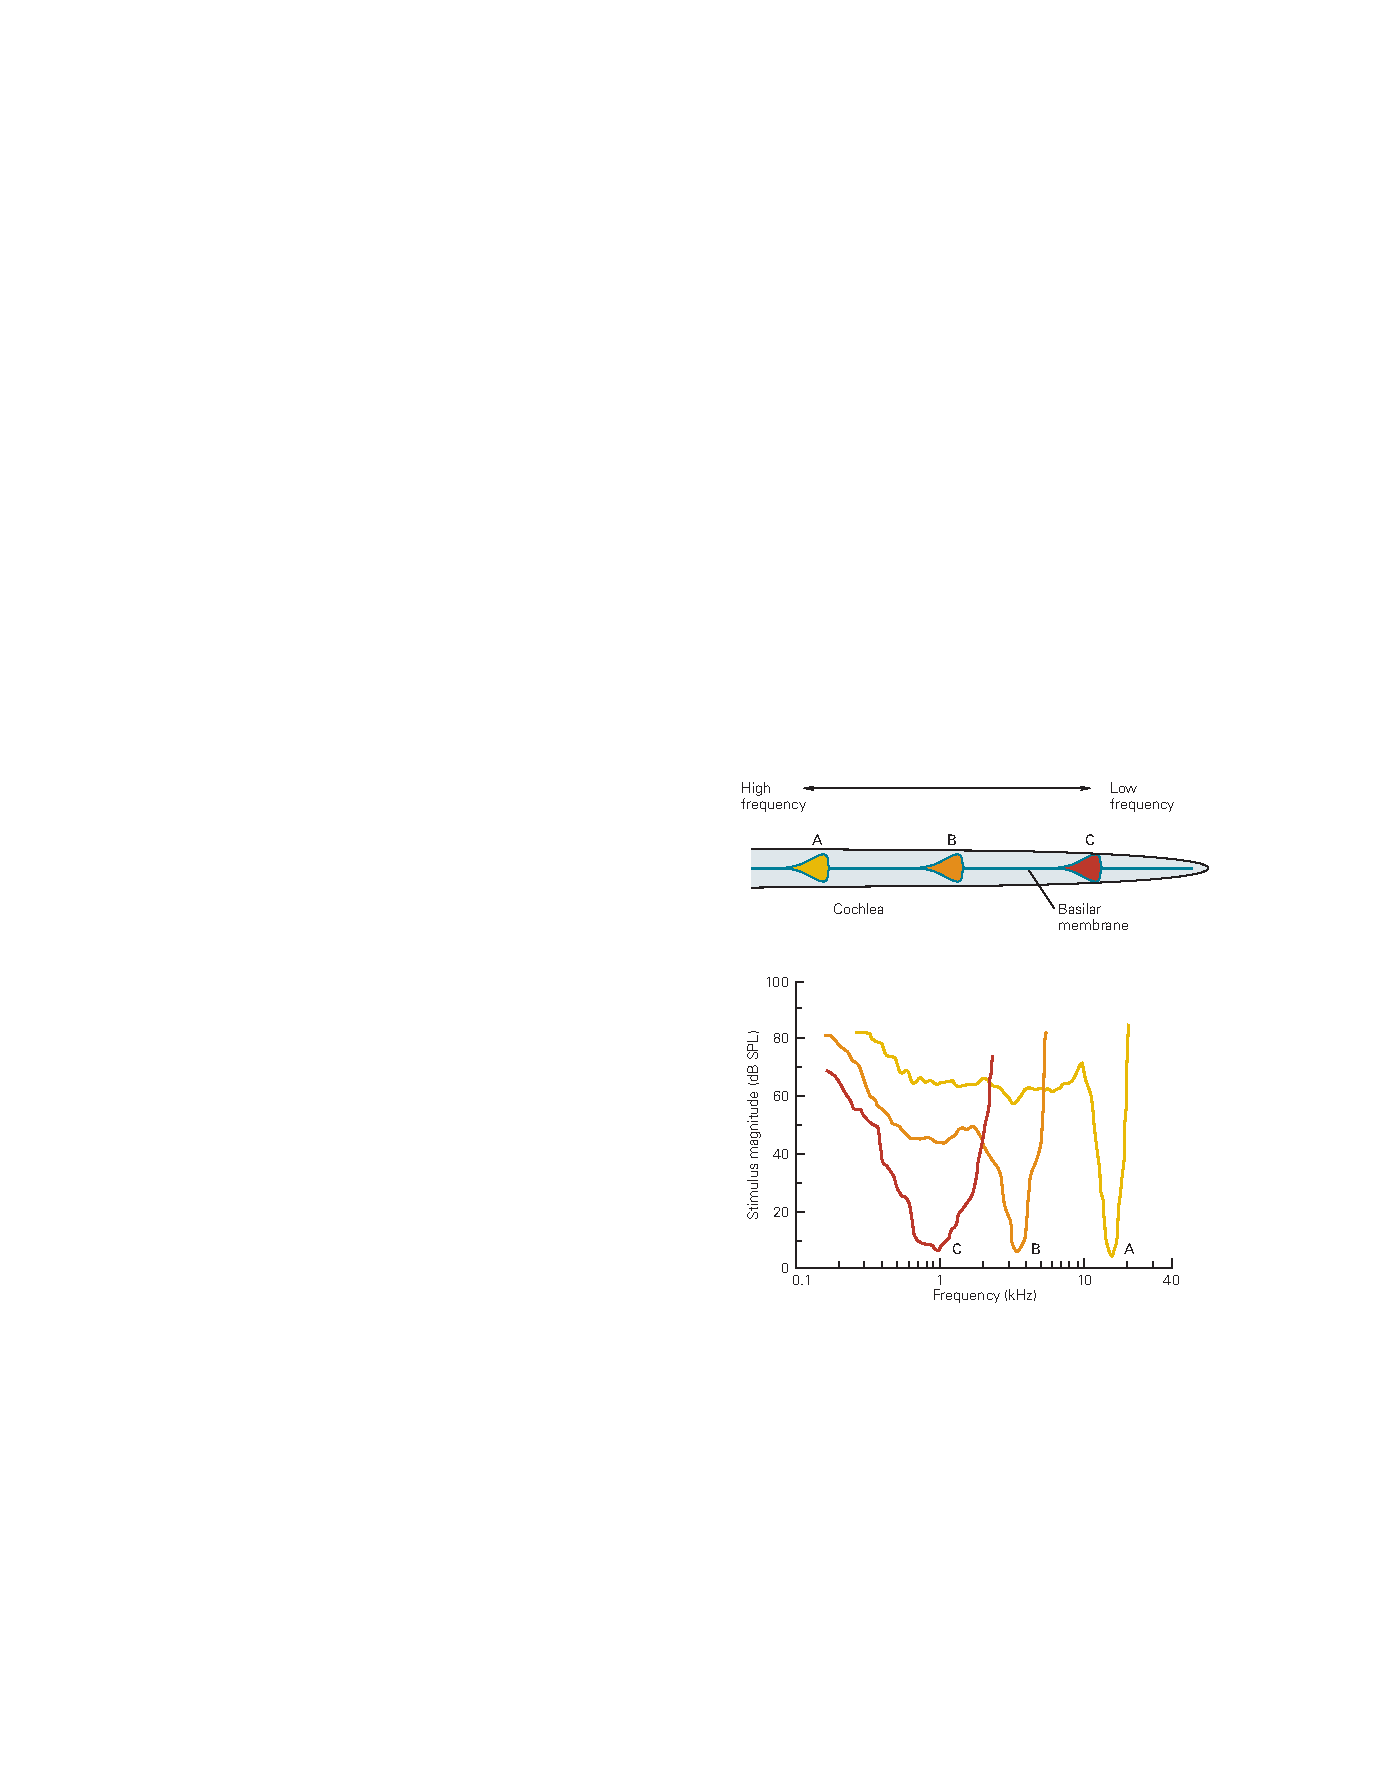
\includegraphics[width=0.5\linewidth]{chap26/fig_26_11}
	\caption{耳蜗毛细胞的调谐曲线。 为了构建一条曲线,实验者以多个频率呈现声音。 在每个频率下,都会调整刺激强度,直到细胞产生标准响应,此处为 1 mV。 因此,该曲线反映了细胞在一定频率范围内的刺激阈值。 每个细胞对特定频率最敏感,即其特征频率。 随着刺激频率的升高或降低,阈值迅速上升——灵敏度迅速下降。 特征频率取决于毛细胞沿耳蜗纵轴的位置。 (经许可转载自 Kiang 1980。版权所有 © 1980 美国声学协会。)}
	\label{fig:26_11}
\end{figure}

就像音叉的共振频率取决于其叉齿的大小一样,发束的高度沿音调轴系统地变化。 对低频刺激有反应的毛细胞具有最高的束,而对最高频率信号有反应的毛细胞具有最短的束。 例如,在人类耳蜗中,特征频率为 20 kHz 的内毛细胞带有一个 4 μm 的毛束。 在相反的极端,对 20 Hz 刺激敏感的细胞具有超过 7 μm 高的束。 外毛细胞观察到类似的形态梯度,补充了基底膜完成的外在调节。

\subsection{毛细胞适应持续刺激}
尽管毛发束的生长非常精确,但它无法以敏感的转导装置始终完美地处于其最大机械敏感性位置的方式发展。 一些机制必须通过调整门控弹簧来补偿发育不规则以及环境变化,以便转导通道对束静止位置的微弱刺激作出反应。 为确保这一点,适应过程会不断重置发束的机械灵敏度范围。 作为适应的结果,毛细胞可以保持对瞬态刺激的高度敏感,同时拒绝一百万倍的静态输入。

适应表现为在毛束长期偏转期间受体电位逐渐降低(图 \ref{fig:26_12})。 
这个过程不是脱敏,因为受体的反应持续存在。 
相反,在长时间的步进刺激期间,初始受体电位和束位置之间的 S 形关系会向应用刺激的方向移动。 
结果,毛细胞的膜电位逐渐恢复到接近其静止值。 然而,适应是不完整的; 膜电位和束位置之间的关系偏移了大约 80\% 的偏转位置。

\begin{figure}[htbp]
	\centering
	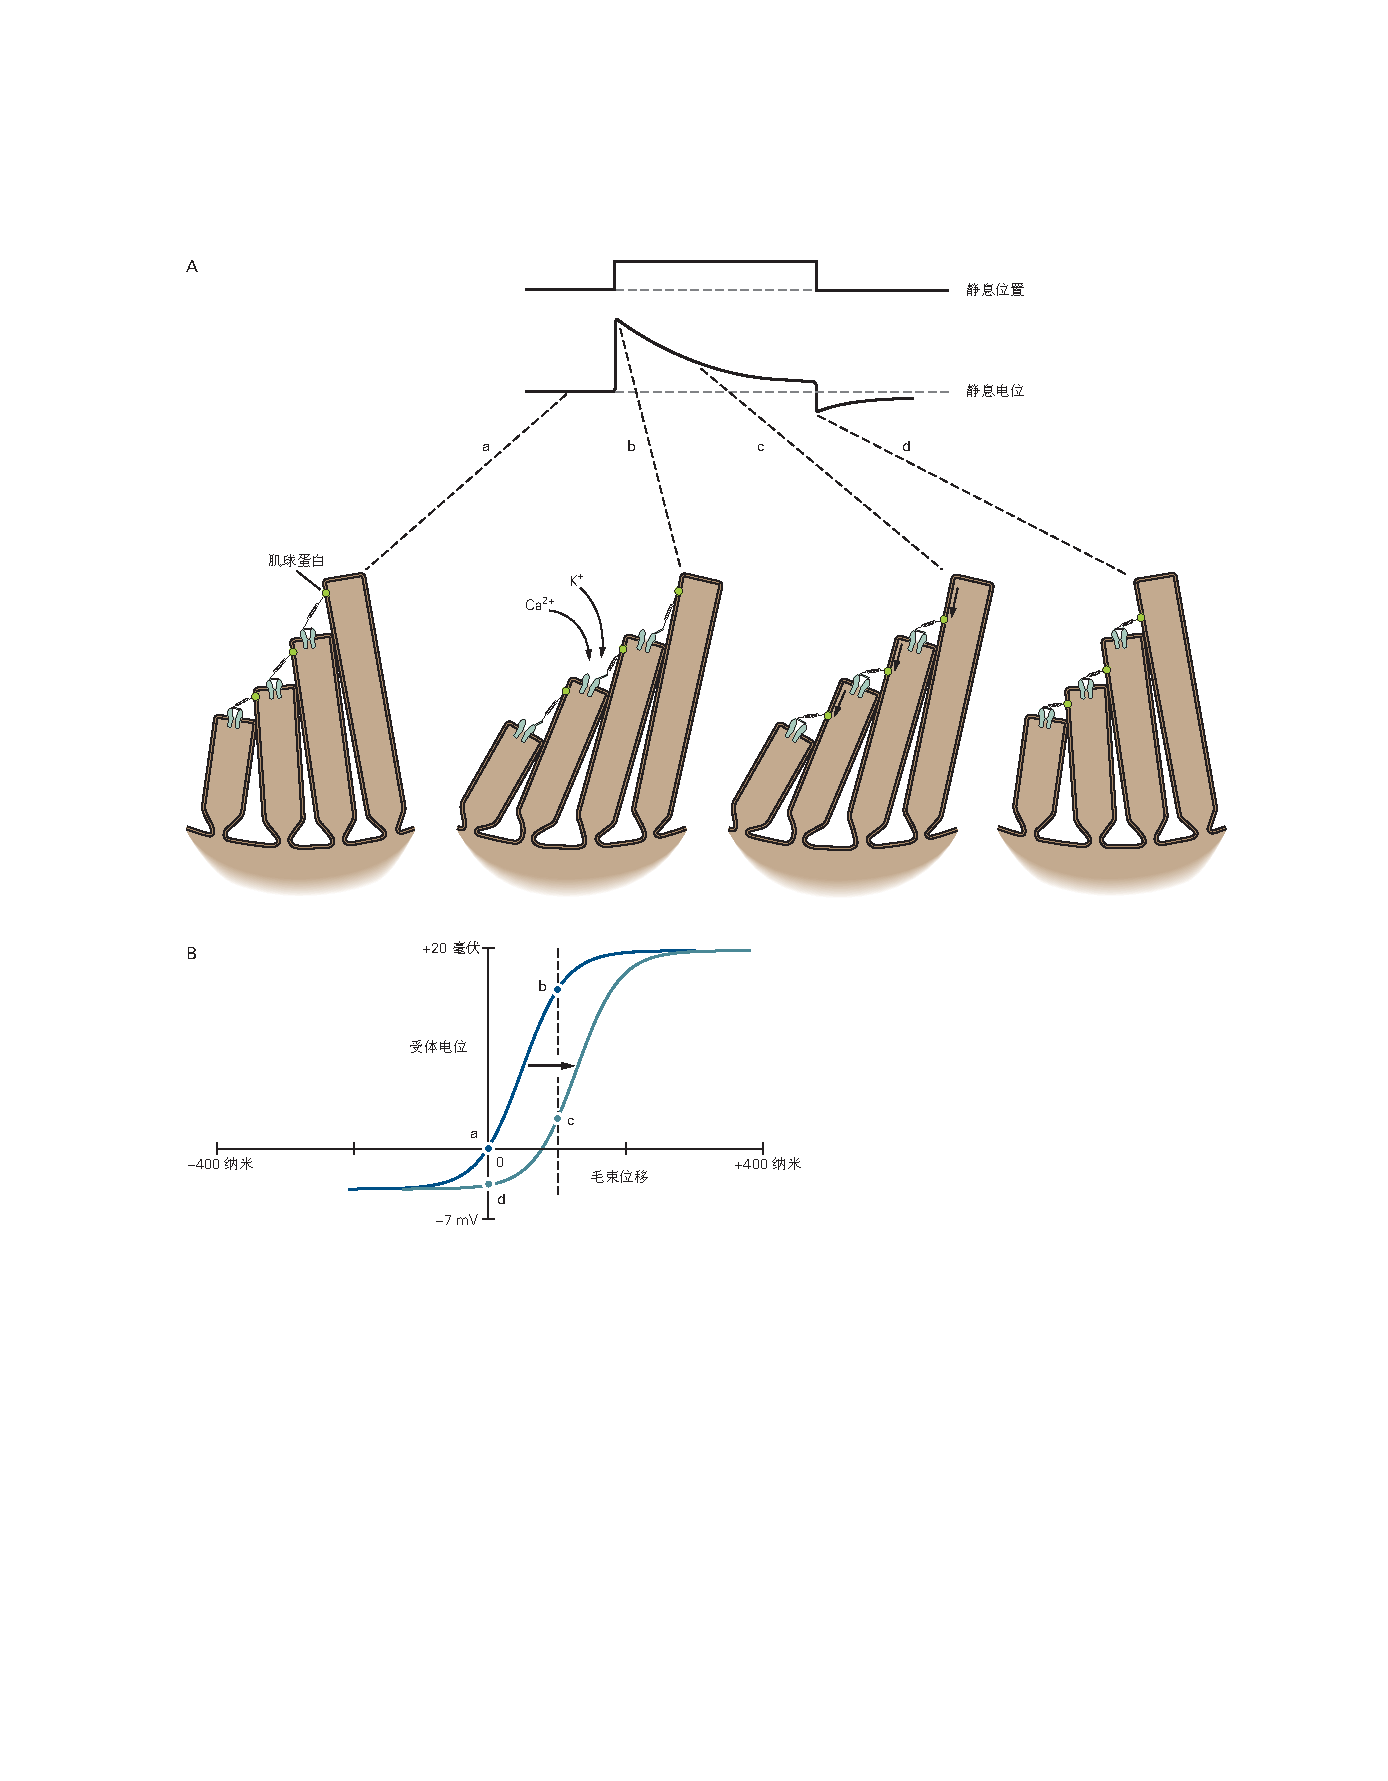
\includegraphics[width=0.95\linewidth]{chap26/fig_26_12}
	\caption{毛细胞中机械电转导的适应。 A. 发束在正方向(上部迹线)上的长时间偏转引起初始去极化,然后下降到平台和刺激停止时的下冲(下部迹线)。 四个示意性毛细胞束说明了转导通道在 (a) 之前和所示适应阶段 (b–d) 期间的状态。 最初,刺激会增加尖端连接(第二束)的张力,从而打开转导通道。 然而,随着刺激的继续,尖端连接的上部附件被认为会滑下静纤毛,从而使每个通道在适应过程中关闭(第三束)。 发束在负方向上的长时间偏转会引起互补反应。 细胞起初轻微超极化,但在刺激结束时显示反弹去极化; 当肌球蛋白分子主动拉起链接的上部插入时,张力恢复到最初松弛的尖端链接。 B. 随着适应的进行,毛细胞位移与毛细胞受体电位之间的S形关系沿横坐标向右移动,向新的毛束位置(虚线)方向移动,曲线的变化不大 形状或振幅。 这种转变解释了为什么受体电位会随着时间的推移而降低,如状态 b 和 c 之间的 A 所示,从而使毛细胞的膜电位恢复到接近其在没有刺激时的值。 这一结果意味着,在存在长期刺激的情况下,适应性恢复了对发束小的快速偏转的机械敏感性,否则会使机械电转导饱和。 A 中显示的转导通道的四种状态已标记为 (a-d)。 (经许可改编自 Hudspeth 和 Gillespie 1994。)}
	\label{fig:26_12}
\end{figure}


适应是如何发生的? 因为随着适应的进行,发束施加的机械力会发生变化,因此该过程显然涉及对门控弹簧承受的张力的调整。 似乎锚定每个尖端链接上端的结构,即插入斑块,在适应过程中被活性分子马达重新定位(图 \ref{fig:26_12})。 转导通道在关闭状态下本质上更稳定,因为它们会在尖端连接中断时关闭。 因此,还需要一台电机通过不断拉动门控弹簧来保持很大一部分 (10\%–50\%) 的转导通道在静止时打开。 与每个尖端链接的上端相关的几十个肌球蛋白分子被认为通过上升静纤毛的肌动蛋白核心并拉动链接的插入来保持张力。

当刺激步骤增加门控弹簧中的张力时,相关的转导通道打开,允许阳离子流入。 当 Ca2+ 离子在静纤毛细胞质中积累时,它们会减少肌球蛋白分子的向上力,从而缩短门控弹簧。 当弹簧达到其静止张力时,通道的关闭将 Ca2+ 流入减少到其原始水平,恢复肌球蛋白向上的力和弹簧中的向下张力之间的平衡。

发束至少包含五种肌球蛋白亚型,肌球蛋白是与肌动蛋白丝运动相关的运动分子(第 \ref{chap:chap31} 章)。 在前庭毛细胞中,免疫组织化学研究和定点诱变表明肌球蛋白 1c 参与适应。 在耳蜗毛细胞中,肌球蛋白 1c 在适应中的作用仍然难以捉摸。 另一种运动蛋白,肌球蛋白 7a,存在于尖端连接的上插入点附近,相应基因 (USH1B) 的突变与耳聋有关。 肌球蛋白 7a 缺陷的毛细胞束杂乱无章,表明该马达至少参与了毛束发育。

如果只是设置转导装置的工作点,适应可以在比声刺激周期慢得多的时间尺度上运行。 这是响应发束大偏转的情况,当内淋巴沐浴发束时,适应时间常数约为 20 毫秒或更多。 这种缓慢的适应与由三磷酸腺苷 (ATP) 的循环水解驱动的基于肌球蛋白的马达的活动相容。 然而,在被小幅度的兴奋性步进刺激拉开后,转导通道以小于 1 毫秒的典型时间尺度重新关闭,因此足够短以与听觉频率兼容。 目前的模型假设通过转导通道进入毛细胞的 Ca2+ 离子与通道孔结合或附近,从而在能量上有利于通道关闭。 这种快速适应的动力学沿着听觉器官的音调轴系统地变化,表明适应可能有助于设定毛细胞最大响应的特征频率。 此外,通道门控和尖端连接张力之间的相互关系意味着自适应通道重排会引起驱动主动发束运动的内力。 因此,适应的机械相关性提供了可以增强对毛细胞刺激的反馈。

\subsection{声能在耳蜗中被机械放大}
内耳面临有效运作的一个重要障碍:声刺激中的大部分能量用于克服耳蜗液体对毛细胞和基底膜运动的阻尼作用,而不是用于刺激毛细胞。 耳蜗的灵敏度太高,听觉频率选择性太强,不可能仅由内耳的被动机械特性引起。 因此,耳蜗必须具有某种主动放大声能的方式。

放大发生在耳蜗中的一个迹象来自于用灵敏的激光干涉仪测量基底膜的运动。 在用低级声音刺激的准备中,基底膜运动高度依赖于频率。 移动在进行测量的位置的适当频率(特征频率)处最大,但在更高或更低的频率处突然下降。 然而,随着声级的增加,振动的频率选择性变得不那么尖锐; 幅度和频率之间关系的峰值变宽。 此外,膜对声音的敏感性(定义为每单位声压的振动幅度)急剧下降。 当以特征频率刺激时,基底膜运动对 80 dB SPL 刺激的敏感性小于 10 dB SPL 刺激的 1\%。 基底膜显示出压缩非线性,可适应声压的百万倍变化,声压将可听声音 (0–120 dB SPL) 表征为仅两到三个数量级的振动幅度 (±0.3–300 nm)。 在被动耳蜗的建模研究中预测的灵敏度和频率选择性与在高水平刺激下观察到的灵敏度和频率选择性相对应。 这一结果表明,在特征频率的低水平刺激期间,基底膜的运动增强了 100 倍以上,但随着刺激强度的增加,这种增强逐渐减弱。 因此,放大将听力阈值降低了 40 到 50 dB SPL 以上。


除了这种间接证据外,实验观察也支持耳蜗包含机械放大器的观点。 当正常人耳受到咔哒声刺激时,该耳朵会在几毫秒内发出一到几个可测量的声音脉冲(图 \ref{fig:26_13} A)。 
因为它们可以携带比刺激更多的能量,所以这些所谓的诱发耳声发射不能简单地是回声; 
它们代表由声刺激触发的耳蜗发射的机械能。 
根据与耳蜗放大相关的压缩非线性,发射的相对水平随着刺激水平而降低。

\begin{figure}[htbp]
	\centering
	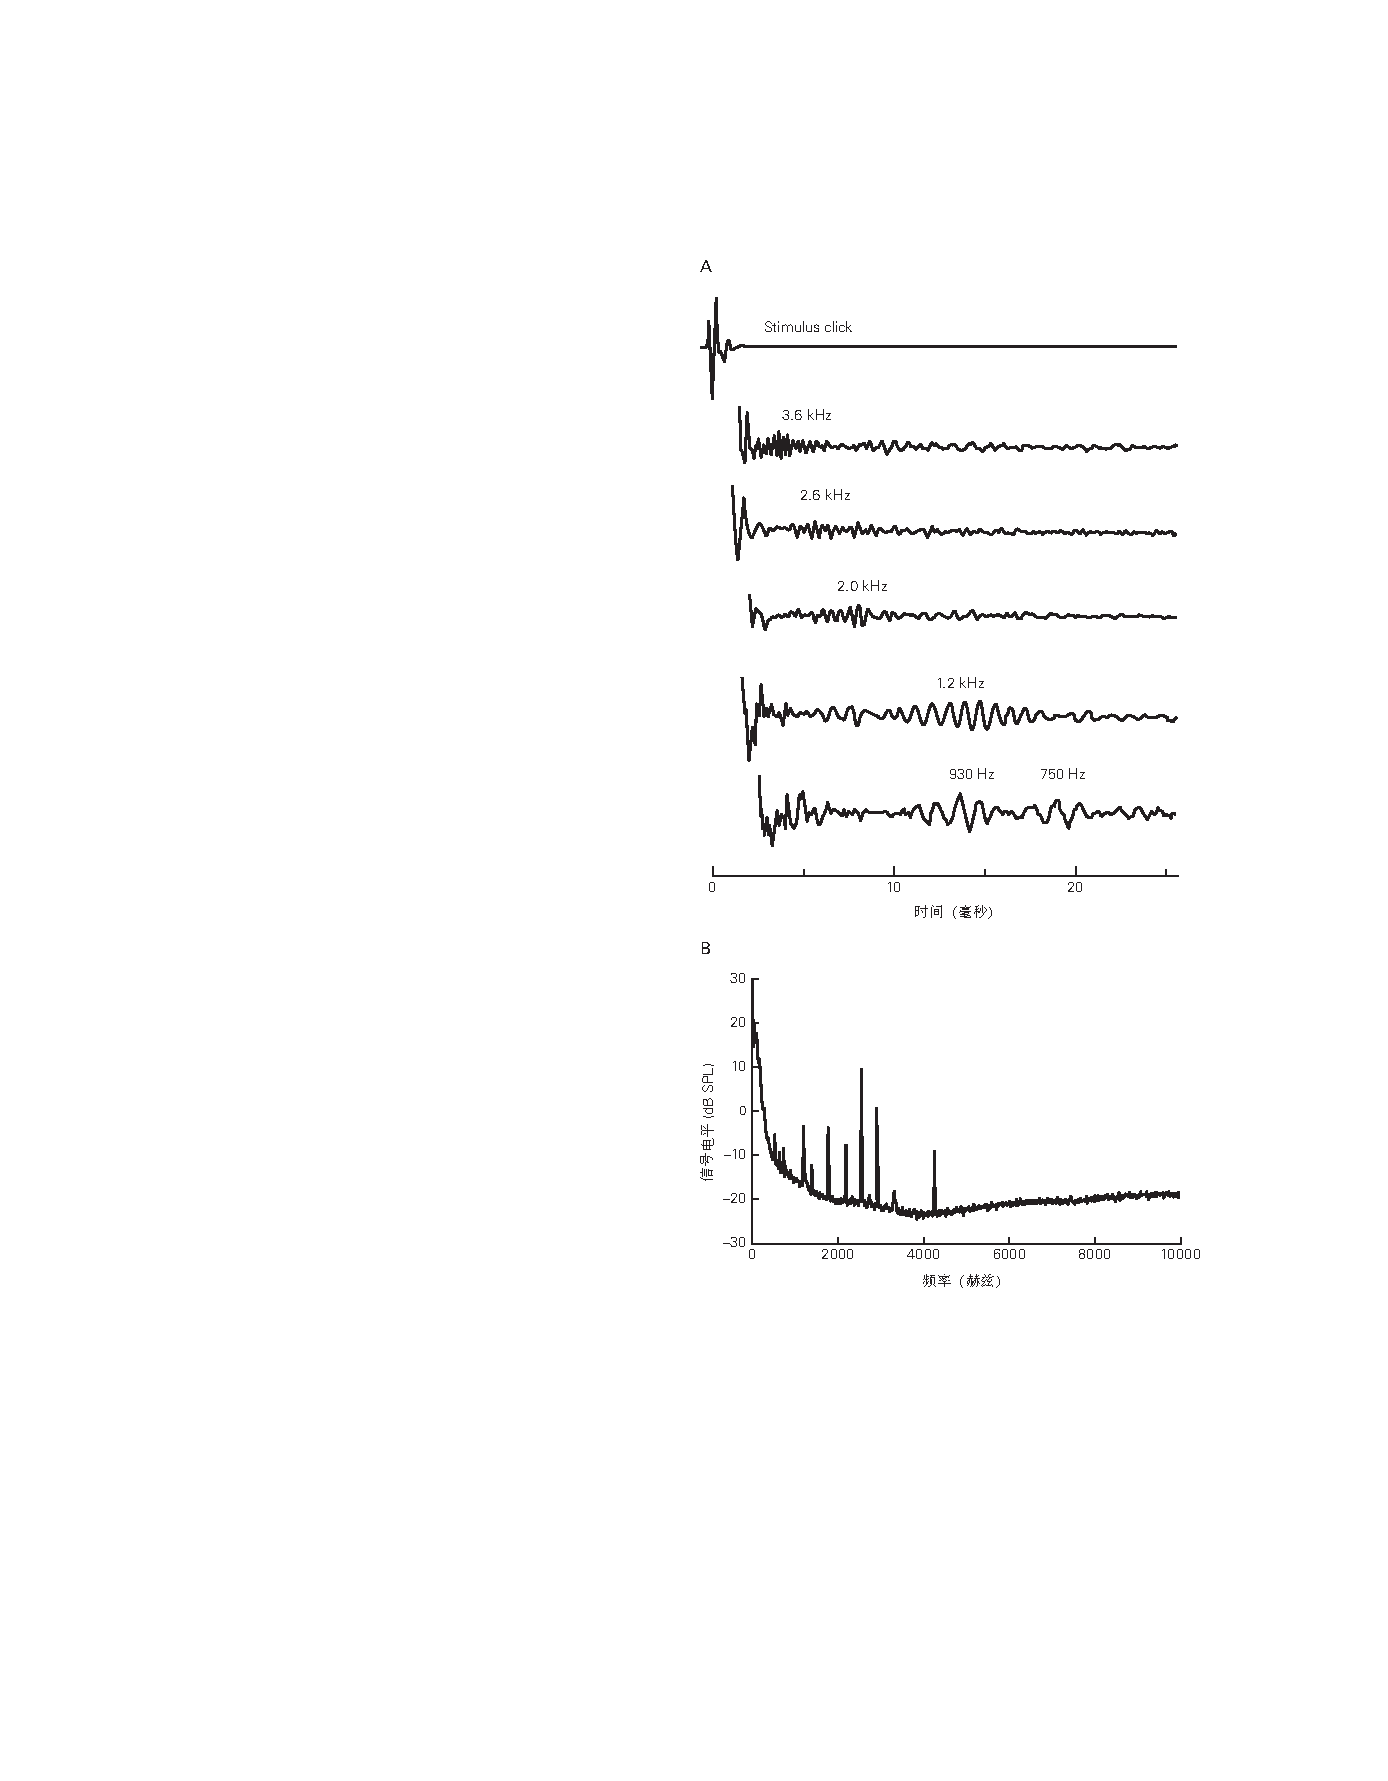
\includegraphics[width=0.5\linewidth]{chap26/fig_26_13}
	\caption{耳蜗主动发出声音。 A. 记录显示从五个人类受试者的耳朵中诱发的耳声发射。 通过微型扬声器向每只耳朵播放短暂的咔嗒声(顶部轨迹)。 几毫秒后,外耳道中的一个微型麦克风检测到从耳朵发出的一次或多次声音爆发。 (经许可改编自 Wilson 1980。版权所有 © 1980 Elsevier B.V.) B. 在适当安静的录音条件下,大多数正常人耳都会发生自发性耳声发射。 该频谱显示了来自一只耳朵的六个突出发射和几个较小发射的声功率。 (经许可转载自 Murphy 等人,1995 年。版权所有 © 1995,美国声学协会。)}
	\label{fig:26_13}
\end{figure}


耳蜗主动放大的一个更引人注目的表现是自发性耳声发射。 当使用灵敏度合适的麦克风在安静环境中测量受试者耳道中的声压时,至少 70\% 的正常人耳会持续发出一种或多种纯音(图 26-13B)。 虽然这些声音通常太微弱以至于其他人无法直接听到,但医生报告说实际上可以听到新生儿耳朵发出的声音!

诱发和自发耳声发射的来源是什么,因此可能也是耳蜗放大的来源? 几行证据表明外毛细胞是增强耳蜗灵敏度和频率选择性的元素,因此充当放大的马达。 广泛支配内毛细胞的传入神经纤维与外毛细胞的接触极少(图 \ref{fig:26_4})。 相反,外毛细胞接受广泛的传出神经支配,激活后会降低耳蜗敏感性和频率辨别力。 
此外,当受到电刺激时,孤立的外毛细胞会表现出独特的电动现象:细胞体在去极化时缩短几微米,在超极化时伸长(图 \ref{fig:26_14})。 
这种响应可以在超过 80 kHz 的频率下发生,这对于假设有助于高频听力的过程来说是一个有吸引力的特征。

\begin{figure}[htbp]
	\centering
	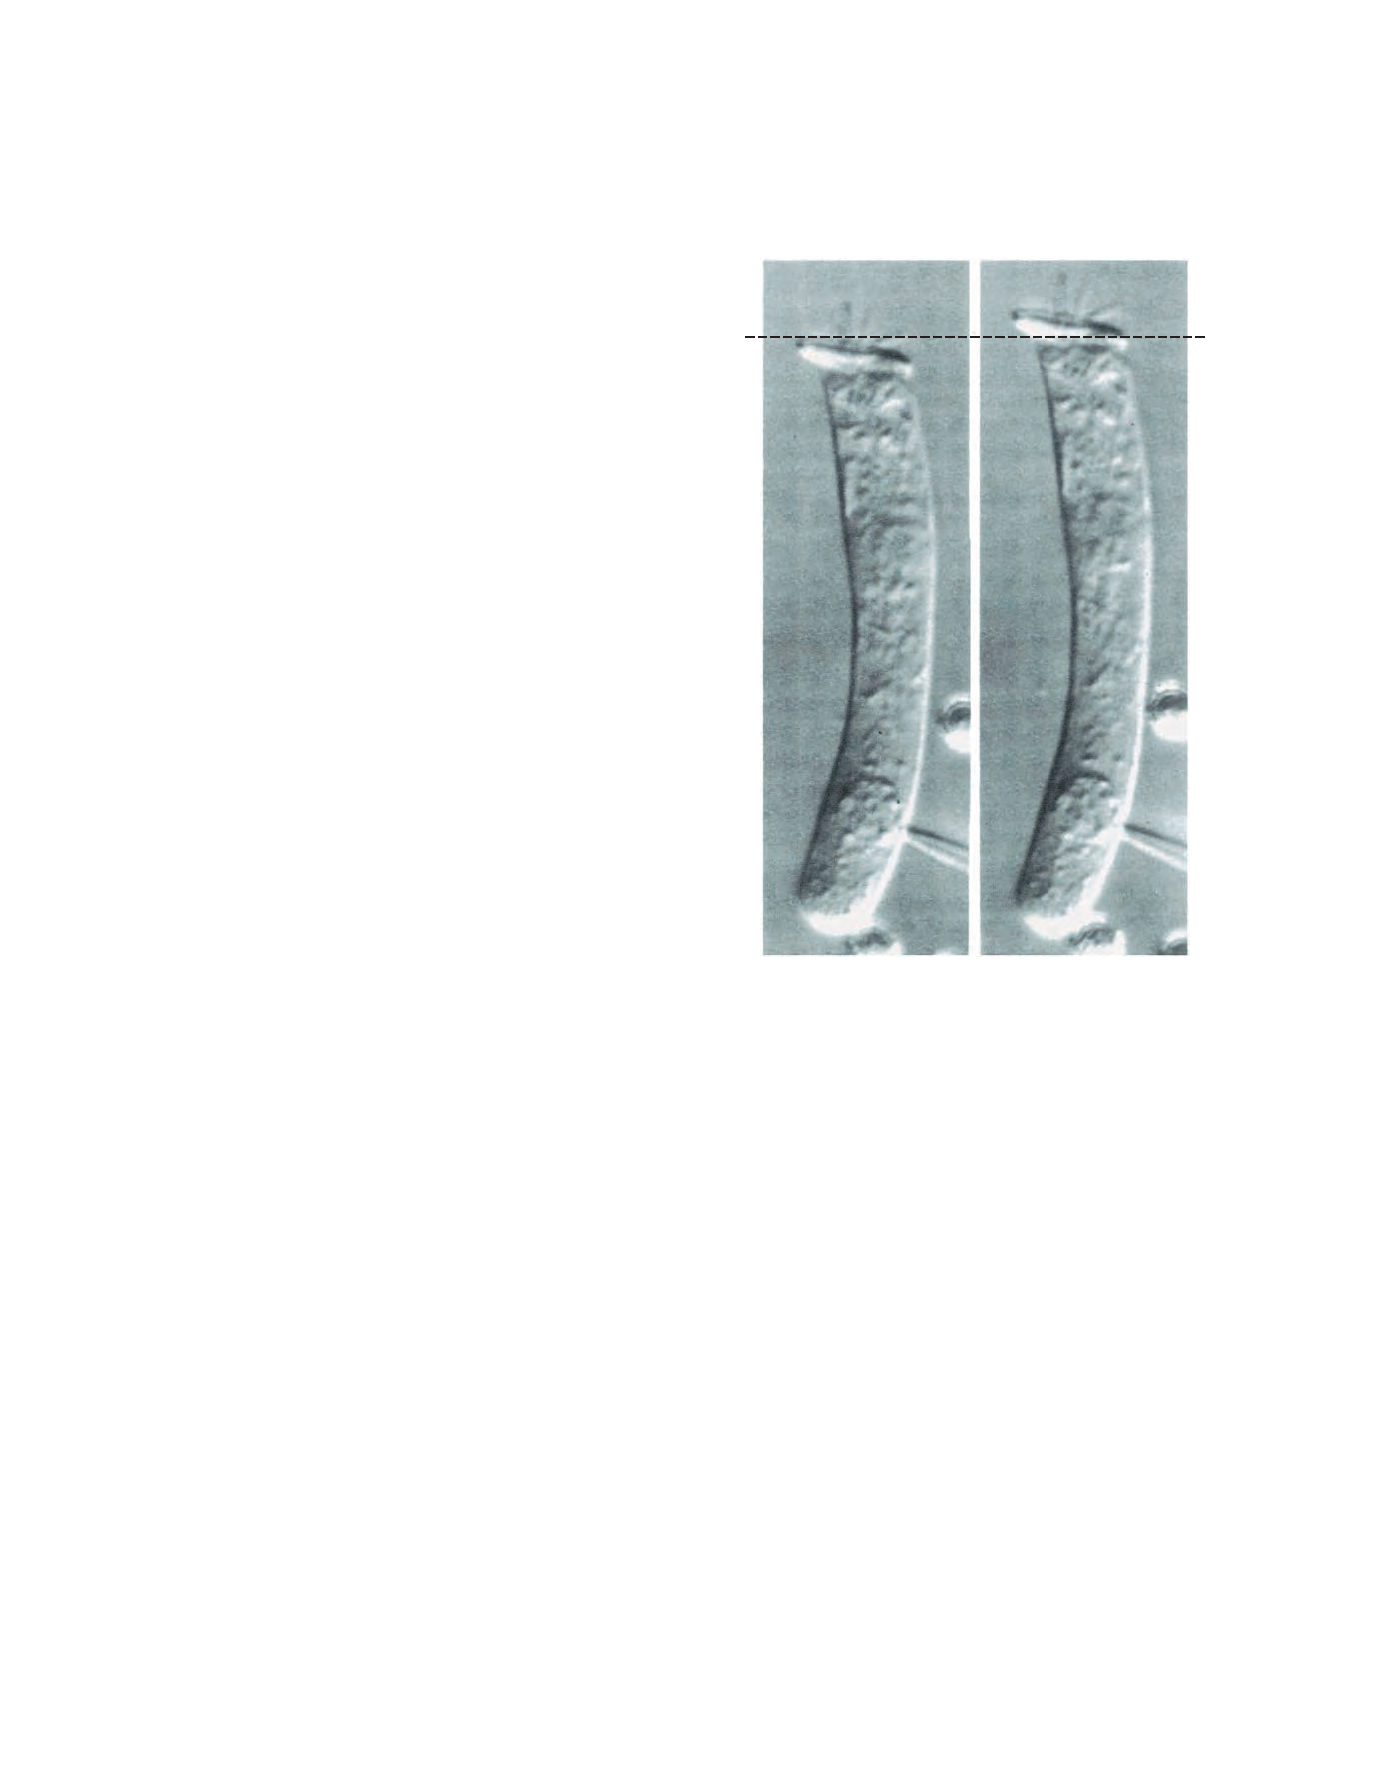
\includegraphics[width=0.5\linewidth]{chap26/fig_26_14}
	\caption{外毛细胞的电压诱导运动。 一个孤立的外毛细胞通过其基部的电极去极化导致细胞体缩短(左); 超极化导致它延长(右)。 外毛细胞的振荡运动可以提供放大基底膜运动的机械能,从而增强人类听觉的灵敏度。 (经许可转载自 Holley 和 Ashmore 1988。)}
	\label{fig:26_14}
\end{figure}


这些运动的能量来自实验施加的电场,而不是来自富含能量的底物(如 ATP)的水解。 当跨膜电场的变化使蛋白质 prestin 的分子重新定向时,就会发生运动。 这些聚集在外毛细胞侧细胞膜中的数百万个分子的协同运动改变了膜的面积,从而改变了细胞的长度。 当外毛细胞将其毛束的机械刺激转化为受体电位时,当细胞体的电压诱导运动增强基底膜运动时,可能会发生耳蜗放大。 与这一假设一致,prestin 的电压敏感性所需的某些氨基酸残基的突变消除了小鼠的活性过程。

由于在缺乏外毛细胞和缺乏高浓度 prestin 的动物物种中也观察到尖锐的频率选择性、高灵敏度和耳声发射,因此电动力不可能是毛细胞机械放大的唯一形式。 除了检测刺激外,发束还具有机械活性并有助于放大。 毛束可以自发地来回运动,这在一些非哺乳动物中已被证明是自发性耳声发射的基础。 在实验条件下,束可以对刺激探针施加力,执行机械功,从而放大输入。 体外实验表明,即使在哺乳动物的耳朵中,活跃的毛束运动也有助于耳蜗的活跃过程。

主动发束运动的速度足以调节至少高达几千赫兹的声音频率的耳声发射。 然而,束是否可以在哺乳动物耳蜗中观察到尖锐的频率选择性和耳声发射的非常高的频率下产生力仍然不确定。 主动发束运动和躯体电动可能协同作用,前者比喻为调谐器和前置放大器,后者则为功率放大器。 或者,发束运动可能在相对较低的频率下占主导地位,但在较高频率下会被电动力所取代。


\subsection{霍普夫分岔为声音检测提供了一般原理}
详细的体内和体外研究揭示了听觉反应的四个主要特征。 首先,主动放大过程降低了检测阈值。 其次,由于放大仅在特征频率附近进行,因此对感觉系统的输入进行了主动过滤,从而增强了频率选择性。 第三,对于特征频率附近的刺激,响应显示压缩非线性,它通过更窄的振动幅度范围代表广泛的刺激水平。 最后,即使在没有刺激的情况下,机械活动也会产生自持振荡,从而导致耳声发射。

这些特征已被认为是主动动力系统(一种临界振荡器)的特征,该系统在振荡不稳定性的边缘运行,称为 Hopf 分岔(方框 26-1)。 它们是通用的:它们不依赖于将系统带到自发振荡边缘的候选机制的亚细胞和分子细节。 主动发束运动在体外证明了 Hopf 分叉这一事实进一步证明了这种机制有助于耳蜗放大。

在此框架内,特征频率由临界振荡器的频率设置。 耳蜗分区可被视为一组主动振荡模块,这些模块由耳蜗流体流体动力学耦合,并且具有沿耳蜗纵轴音调分布的特征频率。 临界振荡的假设有助于行波和耳蜗放大的建模。 这是因为临界振荡器的一般行为可以用一个称为“正常形式”的方程式来描述(方框 26-1)。 临界振荡器非常适合听觉检测,即使其固有的非线性会在响应复杂的声音刺激时产生明显的失真。 事实上,复杂刺激的频率分量之间的非线性干扰似乎是为临界振荡器提供的高灵敏度、尖锐的频率选择性和宽动态范围的听觉检测付出的必要代价。 Hopf 分岔提供了通用属性,这些属性解释了在单个发束、基底膜甚至心理声学中的大量不同实验观察结果。 因此,这种听觉检测的物理原理极大地简化了我们对听觉的理解。 尽管本章主要关注哺乳动物的听觉,但对具有高灵敏度和尖锐频率选择性的听觉的普遍需求对所有陆地脊椎动物的耳朵造成了类似的物理限制。 这些限制导致了耳朵的独立进化,它们具有相似的结构特征,其运作基于相似的物理原理,包括使用临界振荡器来放大声音(方框 26-2)。


\section{毛细胞使用专门的带状突触}

作为感觉受体,毛细胞与感觉神经元形成突触。 每个细胞的基底外侧膜包含几个释放化学神经递质的突触前活性区。 活动区具有四个显着的形态特征(图 \ref{fig:26_16})。

\begin{figure}[htbp]
	\centering
	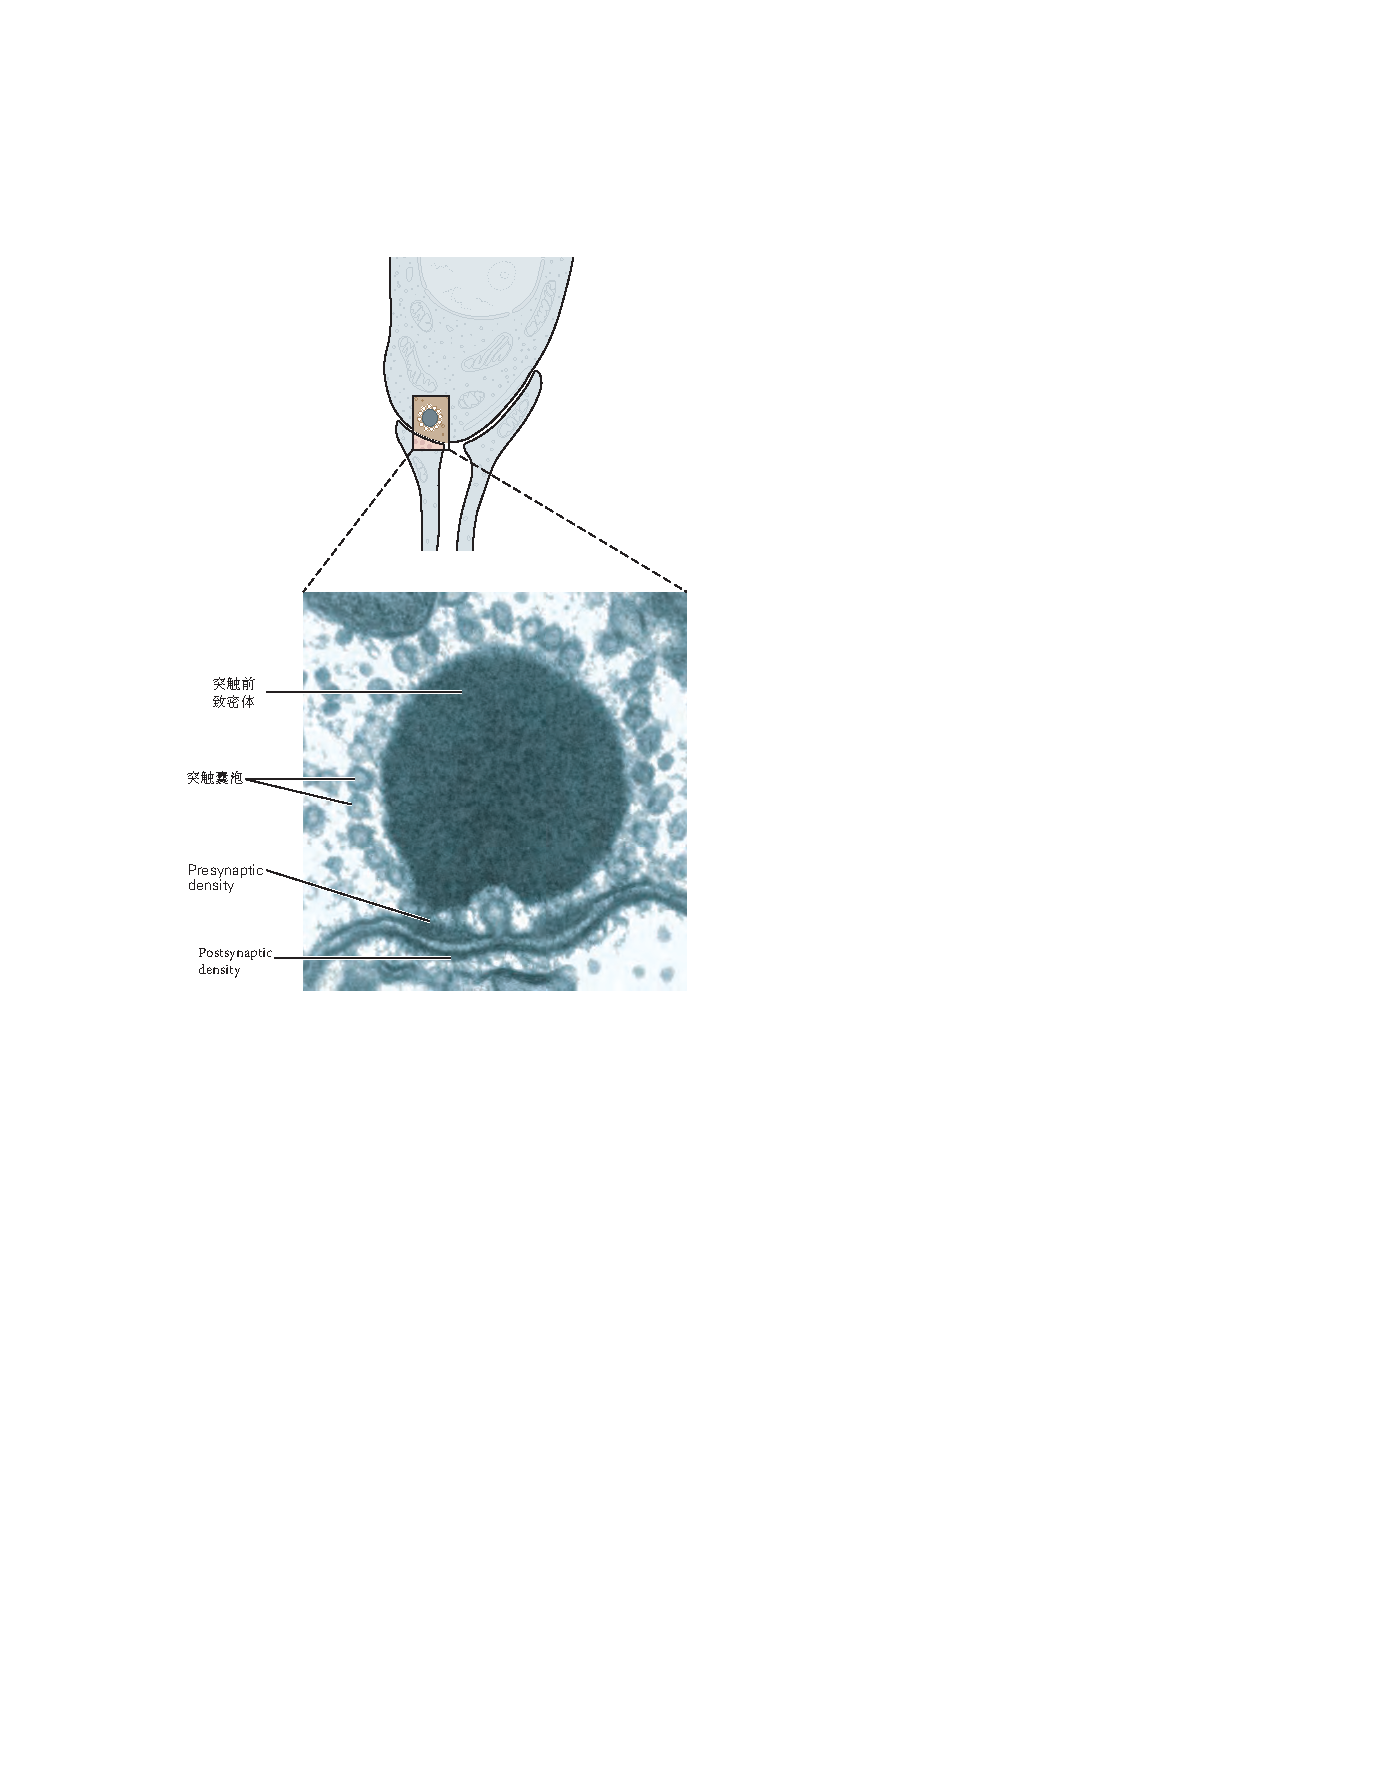
\includegraphics[width=0.5\linewidth]{chap26/fig_26_16}
	\caption{毛细胞的突触前活动区。 这张透射电子显微照片显示了球形突触前致密体或突触带,这是毛细胞突触前活动区的特征。 它被透明的突触小泡包围。 丝带下方是突触前密度,其中一个囊泡正在经历胞吐作用。 适度的突触后密度位于传入终端质膜的内部。 (经许可转载自 Jacobs 和 Hudspeth 1990。)}
	\label{fig:26_16}
\end{figure}

突触前致密体或突触带位于释放位点附近的细胞质中。 这种原纤维结构可以是球形、卵形或扁平形,通常直径为几百纳米。 致密体类似于感光细胞的突触带,代表在许多其他突触中发现的较小突触前密度的专门阐述。 除了与传统突触共有的分子成分外,带状突触还含有大量的肋眼蛋白。

突触前带被清晰的突触小泡包围,每个直径为 35 至 40 nm,它们通过细丝附着在致密体上。 在致密体和突触前细胞膜之间有一个惊人的突触前密度,它由几排短的看起来毛茸茸的物质组成。 在细胞膜内,成排的大颗粒与突触前密度带对齐。 这些颗粒包括参与递质释放的 Ca2+ 通道以及参与非哺乳动物脊椎动物电共振的 K+ 通道。

非哺乳动物实验模型的研究表明,与大多数其他突触(第 \ref{chap:chap15} 章)一样,毛细胞释放递质是由突触前去极化引起的,并且需要从细胞外介质流入 Ca2+。 然而,毛细胞缺乏突触结合蛋白 1 和 2,这些蛋白质作为快速 Ca2+ 传感器的作用可能已被蛋白质 otoferlin 承担,它也促进突触小泡的补充。 虽然谷氨酸是主要的传入神经递质,但也会释放其他物质。

毛细胞的突触前装置有几个不寻常的特征,这些特征是这些细胞信号传递能力的基础。 静止时,内毛细胞不断释放突触递质。 发射器释放的速率可以向上或向下调制,具体取决于毛细胞是分别去极化还是超极化。 与这一观察相一致的是,毛细胞的一些 Ca2+ 通道在静息电位下被激活,提供稳定的 Ca2+ 泄漏,引起未刺激细胞释放递质。 毛细胞突触的另一个不寻常特征是,与光感受器的突触一样,它们必须能够可靠地释放神经递质,以响应仅 100 μV 左右的阈值受体电位。 此功能也取决于突触前 Ca2+ 通道在静息电位时被激活这一事实。

外毛细胞接收来自脑干神经元的输入,形式为基底外侧表面的大环(图 \ref{fig:26_4})。 这种传出系统通过超极化外毛细胞使耳蜗脱敏,从而降低活跃过程。 传出末端包含许多直径约 50 nm 的透明突触小泡,以及少量较大的致密核心小泡。 这些突触的主要递质是乙酰胆碱 (ACh); 降钙素基因相关肽 (CGRP) 也出现在传出末梢,并可能与 ACh 共同释放。 ACh 与由 α9 和 α10 亚基组成的烟碱离子型受体结合,这些亚基对 Ca2+ 以及 Na+ 和 K+ 具有显着的渗透性。 通过这些通道进入的 Ca2+ 激活小电导 Ca2+ 敏感的 K+ 通道(SK 通道),其开放导致长期超极化。 紧靠每个传出末端下方的毛细胞的细胞质拥有一个光滑的内质网池。 这种结构可能参与响应传出刺激进入细胞质的 Ca2+ 的再摄取,从而加速恢复细胞的静息电位。


\section{听觉信息最初通过耳蜗神经流动}
\subsection{螺旋神经节中的双极神经元支配耳蜗毛细胞}
信息从耳蜗毛细胞流向细胞体位于耳蜗神经节中的神经元。 这些双极神经元的中枢过程形成前庭蜗神经(第八颅神经)的耳蜗分裂。 由于该神经节围绕耳蜗骨核呈螺旋形行进,因此也称为螺旋神经节。 大约 30,000 个神经节细胞支配每个内耳的毛细胞。

来自人耳蜗的传入通路反映了内毛细胞和外毛细胞之间的功能区别。 
至少 90\% 的螺旋神经节细胞终止于内毛细胞(图 \ref{fig:26_17})。 
每个轴突只接触一个内毛细胞,但每个细胞将其输出定向到许多神经纤维,平均接近 10 根。这种安排产生了三个重要结果。

\begin{figure}[htbp]
	\centering
	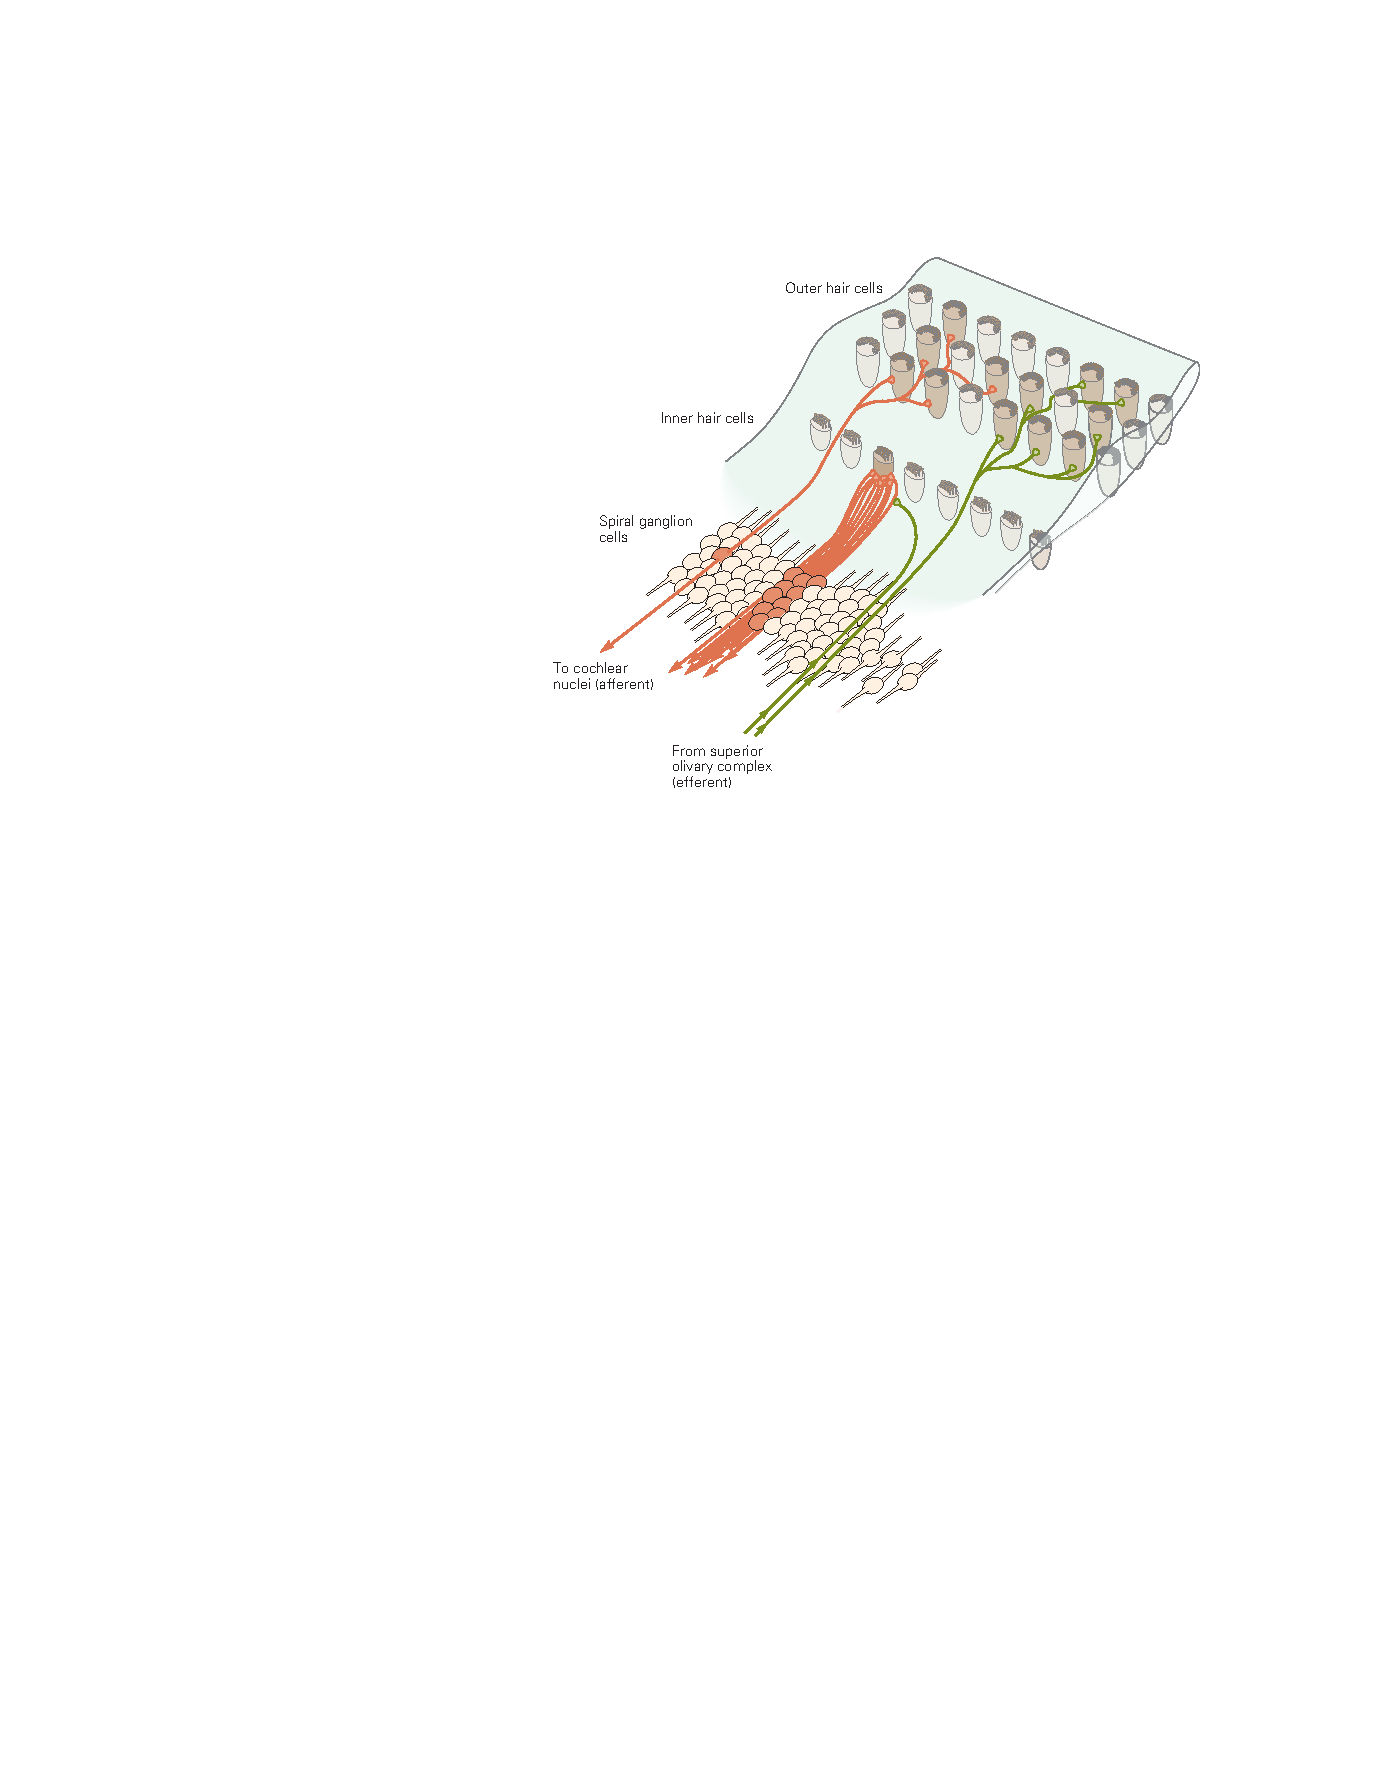
\includegraphics[width=0.65\linewidth]{chap26/fig_26_17}
	\caption{耳蜗毛细胞的神经支配。 耳蜗中的绝大多数感觉轴突(橙色)携带来自内毛细胞的信号,每个内毛细胞构成平均 10 个轴突的唯一输入。 一些小口径的感觉轴突从外毛细胞传递信息。 传出轴突(绿色)主要支配外毛细胞并直接进行。 相比之下,内毛细胞的传出神经支配稀疏,发生在感觉轴突末端。 (经许可改编自 Spoendlin 1974。)}
	\label{fig:26_17}
\end{figure}

首先,产生听力的神经信息几乎完全起源于内毛细胞。 其次,因为每个内毛细胞的输出都被许多传入神经纤维采样,来自一个受体的信息在并行通道中独立编码。 第三,在沿着耳蜗螺旋的任何一点,或在螺旋神经节内的任何位置,每个神经节细胞对突触前毛细胞的特征频率的刺激反应最好。 因此,听觉神经通路的音调组织从尽可能早的位置开始,紧接突触后到内毛细胞。

相对较少的耳蜗神经节细胞与外毛细胞接触,并且每个这样的神经元将分支末端延伸至许多外毛细胞。 虽然已知从外毛细胞接收输入的神经节细胞会投射到中枢神经系统,但这些神经元太少以至于无法确定它们的投射是否对声音分析有重大贡献。

耳蜗毛细胞的传出和传入连接模式是互补的。 成熟的内毛细胞不接受传出输入; 然而,就在这些细胞下方,传出轴突末端和传入神经纤维末端之间存在广泛的轴突-轴突突触接触。 相反,其他传出神经与其基底外侧表面的外毛细胞有广泛的联系。 每个外毛细胞都从几个大的传出终端接收输入,这些传出终端占据了细胞基部和相关支持细胞之间的大部分空间,为传入终端留下的空间很小。



\subsection{耳蜗神经纤维编码刺激频率和水平}
耳蜗神经中轴突的声学敏感性反映了螺旋神经节细胞与毛细胞的连接模式。 每个轴突对特征频率最敏感。 较低或较高频率的刺激也会引起反应,但仅当出现在较高水平时。 轴突的反应性可能以频率选择性或调谐曲线为特征,该曲线呈 V 形,类似于基底膜运动和毛细胞敏感性曲线(图 \ref{fig:26_11})。 具有不同特征频率的神经纤维的调谐曲线彼此相似但沿频率轴移动。

以分贝 SPL 为单位的声级与耳蜗神经每根纤维的放电率之间的关系近似线性。 由于分贝水平对声压的依赖性,这种关系意味着声压是由神经元活动以对数方式编码的。 在光纤动态范围的上端,非常响亮的声音会使响应饱和。 由于动作电位和随后的不应期各持续近 1 毫秒,因此最大可持续放电率约为每秒 500 个尖峰。

即使在具有相同特征频率的神经纤维中,反应阈值也因轴突而异。 最灵敏的纤维,其响应阈值向下延伸至大约 0 dB SPL,具有高自发活动率的特征,并且在中等强度(大约 30 dB SPL)下产生饱和响应刺激。 在相反的极端,最不敏感的传入纤维几乎没有自发活动和更高的阈值,但以分级方式响应甚至超过 100 dB SPL 的水平。 大多数纤维的活动模式介于这些极端之间。

最低灵敏度的传入神经元接触最靠近耳蜗螺旋轴的内毛细胞表面。 另一方面,最敏感的传入神经元接触毛细胞的另一侧。 因此,每个内毛细胞的多重神经支配并不是多余的。 相反,来自给定毛细胞的输出被定向到具有不同灵敏度和动态范围的平行通道。

第八对脑神经中纤维的放电模式表现出阶段性和强直性成分。 轻快的发射发生在音调开始时,但随着适应的发生,发射率会在几十毫秒内下降到稳定水平。 
当刺激停止时,在自发放电率逐渐恢复之前,通常会出现短暂的活动停止,时间过程与适应时间相似(图 \ref{fig:26_18})。


\begin{figure}[htbp]
	\centering
	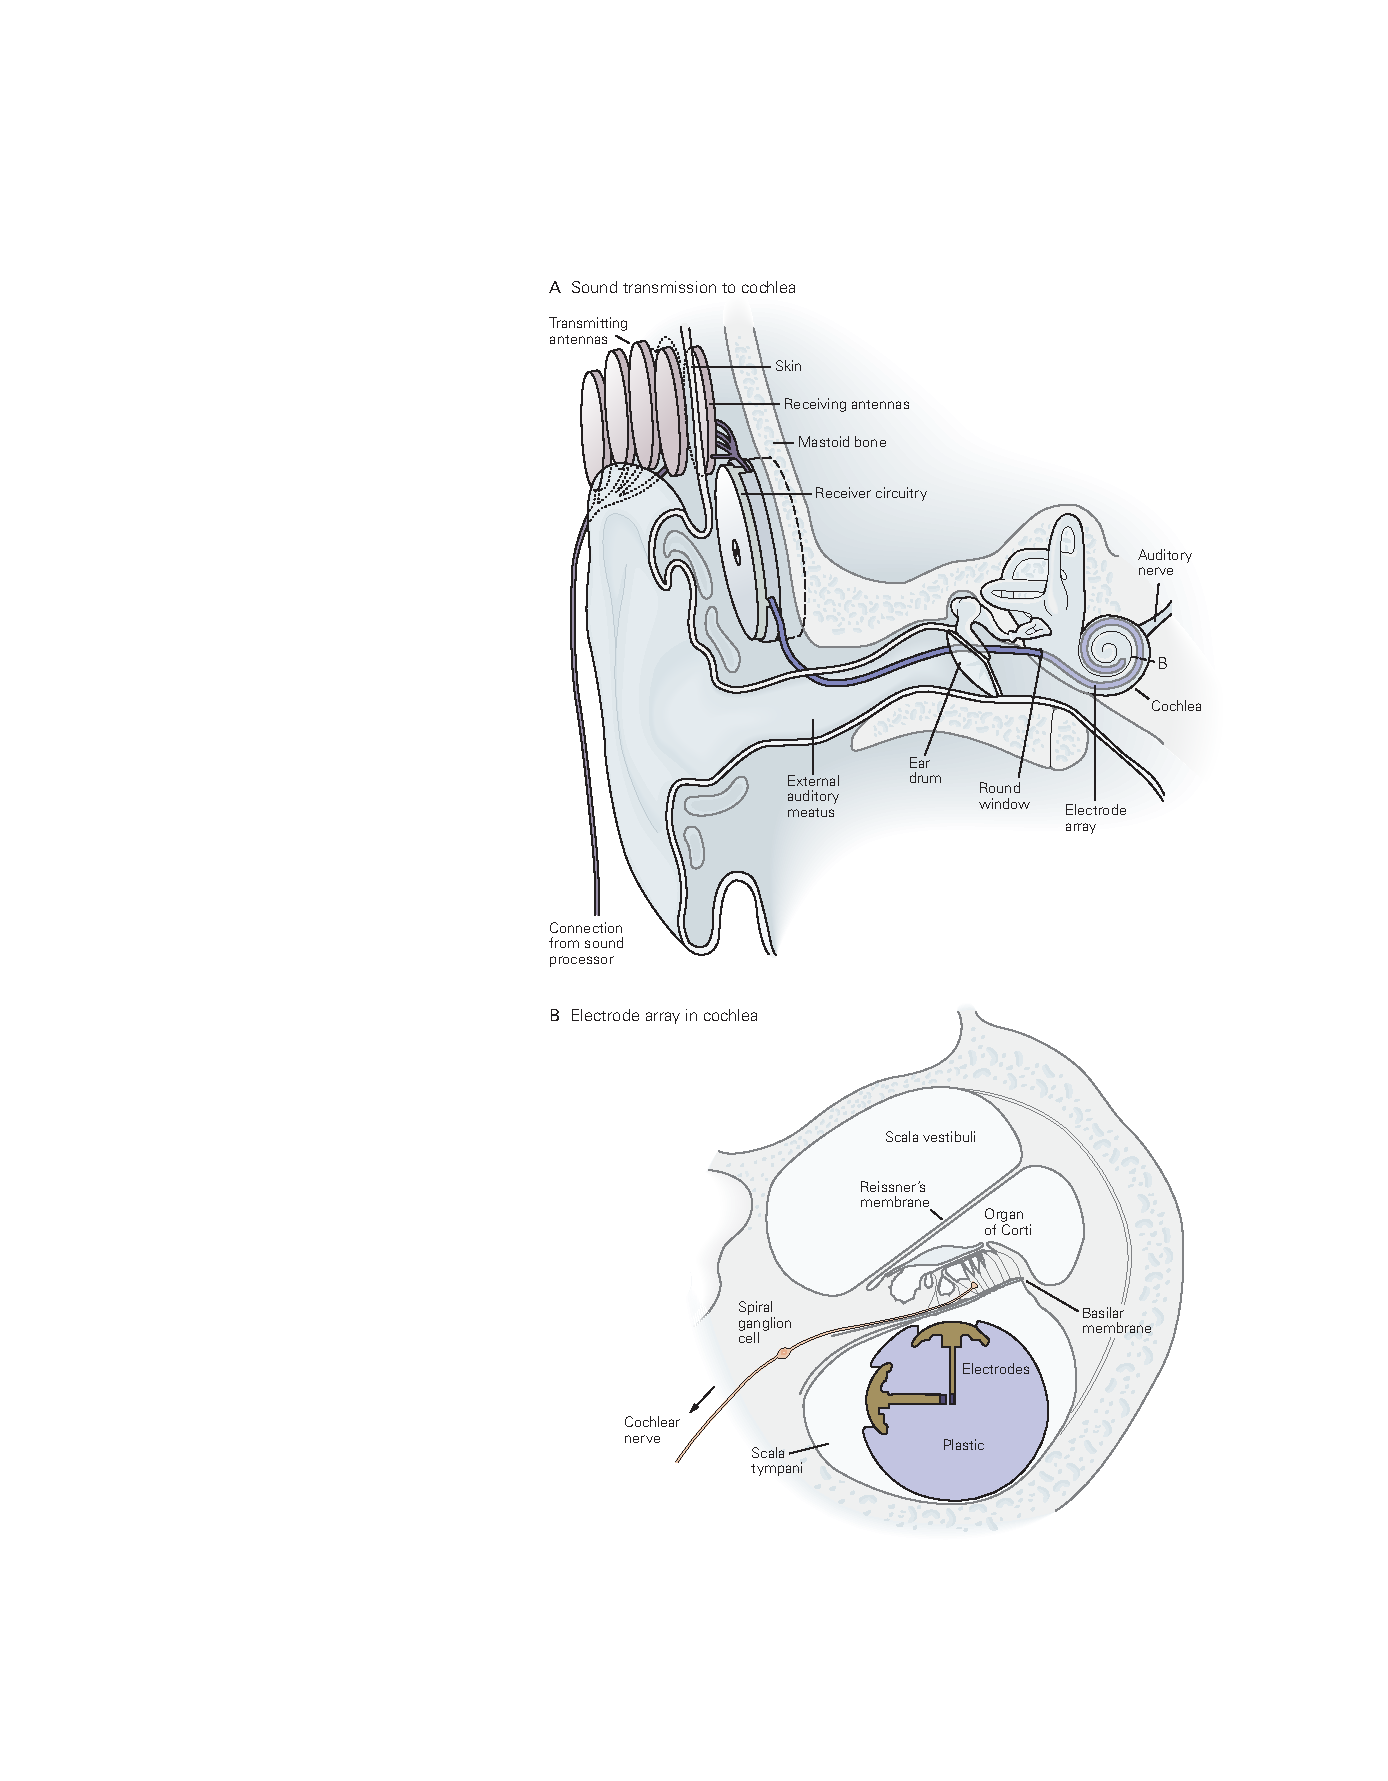
\includegraphics[width=0.5\linewidth]{chap26/fig_26_18}
	\caption{耳蜗神经纤维的放电模式。 耳蜗神经纤维受到大约 5 kHz(细胞的特征频率)的猝发音刺激超过 250 毫秒。 一段平静期后,重复刺激。 直方图显示纤维的平均响应模式作为刺激水平的函数。 样本周期被分成离散的时间段,并显示每个段中出现的尖峰数。 放电的初始阶段性增加与刺激的开始相关。 放电在适应期间的剩余刺激期间继续,但在终止后减少。 当刺激高于阈值 20 dB 或更多时,这种模式很明显。 在刺激之间的间隔期间,活动逐渐恢复到基线。 (经许可改编自 Kiang 1965。)}
	\label{fig:26_18}
\end{figure}


当呈现周期性刺激(例如纯音)时,耳蜗神经纤维的放电模式会编码有关刺激周期性的信息。 例如,在每个刺激周期中,中等强度的相对低频音调可能会在神经纤维中产生一个尖峰。 射击阶段也有定型。 例如,每个动作电位都可能发生在刺激的压缩阶段。 随着刺激频率的升高,刺激最终会变得如此之快,以至于神经纤维无法再逐周期产生动作电位。 然而,直到超过 3 kHz 的频率,锁相仍然存在; 纤维可能仅在每几个刺激周期产生一次动作电位,但它的放电会在刺激周期的特定阶段继续发生。

神经元放电的周期性增强了有关刺激频率的信息。 任何足够水平的纯音都会引起无数耳蜗神经纤维的放电。 那些特征频率与刺激频率一致的纤维在最低刺激水平下做出反应,但对中等强度的刺激反应更加活跃。 其他具有远离刺激的特征频率的神经纤维也有反应,尽管不太强烈。 然而,无论它们的特征频率如何,所有响应纤维都可能显示锁相:每个都倾向于在刺激周期的特定部分发射。

因此,中枢神经系统可以通过两种方式获得有关刺激频率的信息。 首先,有一个位置代码:纤维排列在同位图上,其中位置与特征频率相关。 其次,有一个频率代码:光纤的锁相发射提供了有关刺激频率的信息,至少对于低于 3 kHz 的频率是这样。



\section{感音神经性听力损失很常见,但可以治疗}
无论是轻度还是重度,大多数耳聋都属于感音神经性听力损失的范畴,通常被误称为“神经性耳聋”。 虽然听力损失可能由第八脑神经的直接损伤引起,例如听神经瘤,但耳聋主要源于耳蜗毛细胞及其传入纤维的丧失。

每个人耳蜗中的 16,000 个毛细胞不会被细胞分裂所取代,但必须持续一生。 然而,在两栖动物和鸟类中,可以诱导支持细胞分裂,并诱导它们的后代产生新的毛细胞。 在斑马鱼和鸟类中,一些毛细胞群通过干细胞或支持细胞的活动不断再生。 研究人员最近成功地在体外补充了哺乳动物的毛细胞。 然而,在我们了解如何将毛细胞恢复到柯蒂氏器之前,我们必须应对听力损失。

在过去的几十年里,我们治疗耳聋的能力取得了显着进步。 对于大多数有明显残余听力的患者,助听器可以将声音放大到足以激活幸存的毛细胞的水平。 现代助听器是定制的,以补偿每个人的听力损失,因此该设备可以放大佩戴者最不敏感的频率的声音,同时对仍然可以听到的声音提供很少或根本没有增强。

当一个人的大部分或全部耳蜗毛细胞退化时,再大的放大也无法帮助听力。 但是,可以通过使用人工耳蜗或植入物绕过受损的 Corti 器官来恢复一定程度的听力。 用户佩戴一个紧凑的装置来拾取声音,分离它们的频率成分,并将代表这些成分的电子信号沿着单独的电线转发到位于耳廓后面的小天线。 然后将信号经皮传输到植入颞骨中的接收天线。 从那里,细线将信号传送到适当的电极,这些电极作为阵列植入耳蜗中,沿着鼓阶的不同位置。 
电极的激活会在毛细胞退化后幸存下来的任何附近的轴突中激发动作电位(图 \ref{fig:26_19})。

\begin{figure}[htbp]
	\centering
	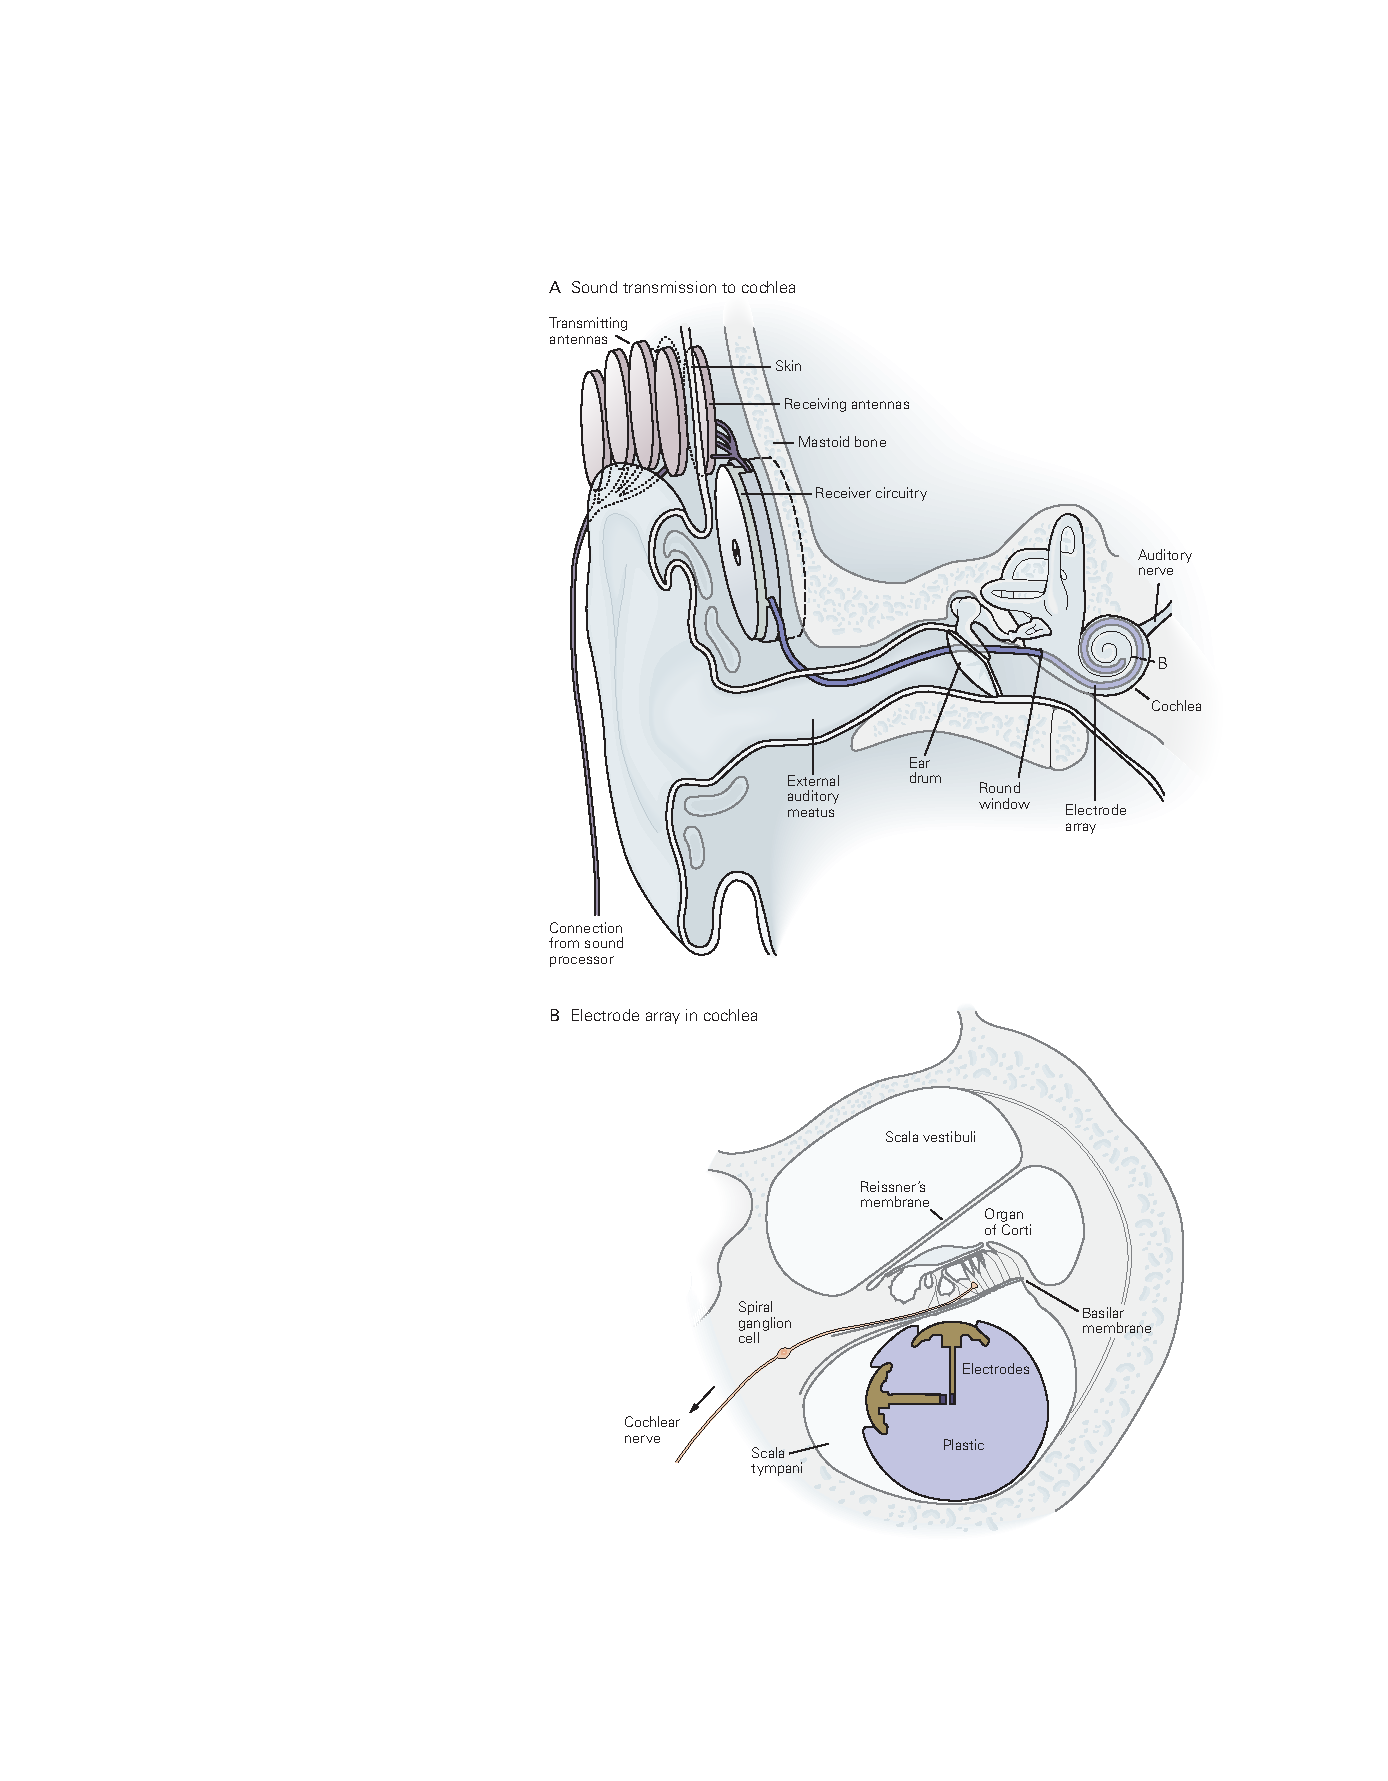
\includegraphics[width=0.7\linewidth]{chap26/fig_26_19}
	\caption{人工耳蜗。 (经许可转载自 Loeb 等人,1983 年。) A. 发射天线接收来自声音处理器的电信号,声音处理器位于受试者的耳廓后面或眼镜框上,并将它们穿过皮肤传输到皮下植入的接收天线 耳廓后面。 然后信号通过细电缆(深紫色)传送到耳蜗中的电极阵列。 B. 耳蜗的横截面显示了鼓阶中电极对的位置。 在电极对之间传递的一部分细胞外电流被附近的耳蜗神经纤维截获,因此被激发并向大脑发送动作电位。}
	\label{fig:26_19}
\end{figure}

人工耳蜗利用沿耳蜗的刺激频率的音调主题表示——位置代码(图 \ref{fig:26_11} 和第 \ref{chap:chap28} 章)。 支配耳蜗每个部分的轴突与特定的、狭窄的频率范围有关。 假体中的每个电极都可以激发一组代表相似频率的神经纤维。 受刺激的神经元然后沿着第八神经将它们的输出转发到中枢神经系统,在中枢神经系统中,这些信号被解释为基底膜上该位置所代表的频率的声音。 大约 20 个电极的阵列可以通过适当地刺激几个神经元簇来模拟复杂的声音。

全球植入人工耳蜗的数量现已接近 350,000。 然而,它们的有效性因人而异。 最好的结果是,在安静的条件下,一个人几乎可以像听力正常的人一样理解语音,甚至可以进行电话交谈。 另一个极端是从假肢中获益甚微的患者,大概是因为电极阵列附近的神经纤维广泛退化。 大多数患者发现他们的假肢很有价值。 即使听力没有完全恢复,这些设备也有助于唇读并提醒患者注意环境中的噪音。

听力损失通常伴随着另一种令人痛苦的症状,即耳鸣或“耳鸣”。 通过干扰注意力和扰乱睡眠,耳鸣会激怒、压抑甚至使受害者发疯。 因为在极少数情况下耳鸣源于听觉通路的病变,例如听神经瘤,所以在神经学诊断中排除此类原因很重要。 然而,大多数耳鸣是特发性的:其原因尚不确定。 越来越多的研究表明压力是一个重要因素。 有些药物也会引发这种情况; 与用于治疗类风湿性关节炎的高剂量奎宁和阿司匹林相关的抗疟药因这一点而臭名昭著。 然而,耳鸣通常发生在受损耳朵不再敏感的高频频率下。 在这些情况下,耳鸣可能反映了传入神经阻滞系统的超敏反应,一种类似于幻肢痛的现象(第 \ref{chap:chap20} 章)。


\section{要点}
1. 听觉始于耳朵对声音的捕捉。 外耳捕获的机械能通过中耳流到耳蜗,在那里引起弹性基底膜振动。 

2. 基底膜支撑着内耳的受体器官——柯蒂氏器,这是一条包含大约 16,000 个机械感觉毛细胞的上皮条带。 毛细胞将基底膜振动转变成受体电位,从而导致感觉神经元放电。 

3. 声音刺激的频率分量由不同的毛细胞在基底膜的不同位置检测到,遵循音调图。 基底膜的机械梯度有助于耳蜗的频率分析。 此外,每个毛细胞都根据其形态、机械和电学特性以特征频率进行调谐,这些特性沿着耳蜗的音调轴连续变化。 

4. 毛细胞的运作速度比其他感觉受体快得多,这使它们能够对某些哺乳动物物种中超过 100 kHz 的声音频率做出反应。 因此,毛细胞中的机械电转导通道直接由机械应变激活。 

5. 每个毛细胞从其顶端表面伸出一簇圆柱形静纤毛——毛束,它作为机械天线工作,响应声音刺激而振动。 转导通道出现在立体纤毛尖端。 它们的开放概率由互连相邻静纤毛的尖端链接中的张力变化调节。 

6. 在感觉受体中独一无二的是,毛细胞放大了它们的输入以增强它们的敏感性,提高它们的频率选择性,并扩大它们可以检测到的刺激水平的范围。 两种形式的细胞运动有助于这一活跃过程。 首先,受体电位会引起外毛细胞胞体的长度变化,这是一种压电的生物模拟,称为电动力。 其次,毛束——毛细胞的机械感应天线——可以自主振动。 

7. 耳朵不仅接收声音而且发出声音称为耳声发射。 自发和诱发的耳声发射是由耳蜗的主动放大过程引起的。 

8. 耳蜗不作为高保真声音接收器; 相反,它引入了有助于声音感知的明显失真。 听觉非线性起源于耳蜗,它优先放大微弱的声音刺激,并构成敏感听力的标志,用于筛查新生儿的听力缺陷。 

9. 如果耳蜗包含活跃的机械模块,每个模块都在振荡不稳定性的边缘——霍普夫分叉——运行,那么在单个发束、基底膜和心理声学水平上的大量实验观察很容易得到解释。 Hopf 分岔提供了听觉检测的一般原理,简化了我们对听觉的理解。 

10. 听觉的进化史表明,各种陆生脊椎动物在很大程度上独立地获得了听觉系统,但它们的灵敏度和频率选择性是相似的。 特别是,哺乳动物和非哺乳动物的耳朵都受益于声音输入的机械放大并显示耳声发射。 哺乳动物与其他群体最显着的不同之处在于它们的听觉范围扩展到 12 至 14 kHz 以上的频率。 

11. 对耳聋遗传形式的分析提供了关于毛细胞功能的数十种关键蛋白质的信息,特别是那些负责机械电转导和毛细胞与听神经纤维之间的突触传递的蛋白质。 尽管这些基因可能成为未来治疗的潜在目标,但目前主要通过助听器或人工耳蜗来治疗感音神经性听力损失。 新策略,例如通过干细胞分化补充毛细胞或螺旋神经节的光遗传学刺激,为听力恢复研究提供了有希望的途径。

%\subsection{选读}
%\subsection{参考文献}